\section{Files}
\subsection{Data}
\sloppy
\subsubsection{Location}
The data from this experiment was saved in the directory 
\verb|/ladd/data2/emma/data/| on the LADD cluster.  The data is physically located on the computer \texttt{ladd02.triumf.ca}. Assuming \texttt{ladd02} is turned on and connected to the network, the data is accessible with the \texttt{emma} user account on any of the LADD cluster servers, such as \texttt{ladd19}, \texttt{ladd20}, or \texttt{ladd21}. The data has been copied to the computer \texttt{lighthall.triumf.ca} and is located in the directory \verb|/Users/lighthall/data/PGAC_test/data|.
A symbolic link to the data directory has been made in the analysis directory with the name \verb|data\|.
\subsubsection{Accessing the data}
The LADD cluster does not use individual usernames. Each group is assigned group login credentials. The login credentials for the EMMA group are given below.
\begin{quote}
\interlinepenalty=1000
  \begin{verbatim}
    username: emma
    password: daq_test2014
  \end{verbatim}
\end{quote}
\vsetlinux
Log onto the LADD cluster using SSH via the servers \texttt{ladd19}, \texttt{ladd20}, or \texttt{ladd21}.  If connecting from offsite,  \texttt{.trifumf.ca} must be appended to the server address. The command for logging onto the cluster follows.
\begin{quote}
  \begin{Verbatim}
ssh -Y emma@ladd19.triumf.ca 
		\end{Verbatim}
\end{quote}
In this example, the \texttt{ladd19} computer is used. The \texttt{-Y} flag is used to enable X11 tunneling in order to view histograms, etc. on the remote computer. In order to view windows on the remote computer, make sure an X Windows program is running on the local computer, for example XQuartz (OS X) or XWin (Windows). After entering this command, you will be prompted for the EMMA account password. Once logged in, the user will start out in the EMMA home directory \verb|\home\emma|.
\subsubsection{Run contents}

The April 2014 experiment started with Run 371 and ended on Run 480.  Of these 110 runs, 69 of them were written to disk. 
The settings of the runs are discussed in Section~\ref{settings_sec}.  
Except where indicated otherwise, all of the data referred to in this section is from Run 480.

%, which was the last run of the experiment.
Run 480 was selected---arbitrarily---because it was the last run of the experiment. The data for this run is contained in five MIDAS files. The duration of the run was 13\,min 25\,sec. After sorting, this run contains about 30,000 events, with 25,000--29,000 in pair-wise coincidence, depending on signals in question. The detector settings for this run were $P=3$\,Torr, $V_\textrm{c}=-80$\,V, $V_\textrm{a}=+435$\,V ($\Delta V=515$\,V).  The beam current for this run was 0.64\,enA ($120\times$ attenuator). It was one of 17 data runs at $P=3$\,Torr. Because of the low beam intensity, Run 480 had the highest $\Delta V$ setting of any other run at $P=3$\,Torr.  For example, it was the only run at $P=3$\,Torr with $V_\textrm{c}$ set to a value other than $-75$\,V.

The April 2015 experiment started with Run 576 and ended with Run 611. Of the 36 runs, data was written to disk for 24 runs. The initial calibration constants were developed for Run 606. The thresholds of every detector channel were optimized before the start of this run and should represent an optimized electronics setup.

\subsection{Readout}
\vsetlinux
The main analysis program is \texttt{ana.cxx}. Four vairations of the readout code have been developed by the author.
References to readout code in the following sections refer to the program \texttt{ana.cxx} currently located in 
\verb|ladd19.triumf.ca:/home/emma/offline/lighthall/rootana/analysis/|.  Here \texttt{ladd19} 
could be replace with any of the computers in the LADD cluster.  This readout program is built upon the minimum working example readout code located in \verb|ladd19.triumf.ca:/home/emma/packages/rootana/examples/|. The readout programs utilize the \texttt{TV1190Data.hxx} class.

\subsubsection{\texttt{ana\_bare.cxx}}
The file  \texttt{ana\_bare.cxx} is a stripped-down minimal working example (``bare bones'') of the readout code. 
The code is run with the command
\begin{quote}
  \begin{Verbatim}
./ana_bare.exe data/run00606sub00000.mid.gz   
\end{Verbatim}
\end{quote}
and output files are saved into the directory \verb|./output/| with the file name \verb|emma_ana_bare_00606.root|.


The structure of the code discussed here applies to the three other readout codes.
The program contains two main functions which are modified for the purposes of calibration and analysis.
At the start of each run, the function \verb|BeginRun()| is called. This code is run once per data set. Here the histograms are defined.

The data are read out using the function \texttt{ProcessMidasEvent()} within the \texttt{TRootanaEventLoop} class. This function is called once per event.
The data are first parsed into channel number and value using the TV1190Data class.   
Once the data is unpacked by \texttt{ProcessMidasEvent}, they are filled into ROOT histograms. 
A number of ``raw'' histogram are filled with uncalibrated data. This is illustrated in the following code box. %\newpage
%\pangram{50}%\hline
\vspace{0.5\baselineskip}
\par\noindent
\begin{minipage}{\linewidth}
  \singlespace
\begin{lstlisting}[caption={Unpack data. Here for a given event, \texttt{chan} is a variable which takes the value of the channel number, %for which an event has been recorded,
 \texttt{counts} records the number hits per channel , \texttt{datum} is an array which stores all of the measurements for a given event,
 and \texttt{hdata} is a raw histogram of counts per channel. }]
//--- Unpack data
for(unsigned int i = 0; i < measurements.size(); i++) { //loop over measurements
   chan = measurements[i].GetChannel();
   counts[chan]++; //"counts" per channel (multi-hit)
   datum[chan][counts[chan]] = measurements[i].GetMeasurement();
   hdata[chan]->Fill(datum[chan][counts[chan]]);//raw data histograms
}
\end{lstlisting}
%\vspace{-1.3\baselineskip}
\end{minipage}


\subsubsection{\texttt{ana.cxx}}
The file  \texttt{ana\_bare.cxx} is a stripped-down minimal working example (``bare bones'') of the readout code. 
The code is run with the command
\begin{quote}
  \begin{Verbatim}
./ana.exe data/run00606sub00000.mid.gz   
\end{Verbatim}
\end{quote}
and output files are saved into the directory \verb|./output/| with the file name \verb|emma_ana_00606.root|.
%the function \verb|BeginRun()| and 
Calibration parameters are read in with a simple file I/O subroutine. The calibration constants are stored in text files located in the directory
\verb|ladd19.triumf.ca:/home/emma/offline/lighthall/rootana/analysis/cal/|. Default calibration constants were developed for runs 430, 480, and 606 which were the most thoroughly analyzed runs. In cases where these default values do not properly calibrate the data, additional calibration constants were developed on a run-by-run basis.

%\hline
%\pangram{50}
%Here for a given event, \texttt{chan} is a variable which takes the value of the channel number, %for which an event has been recorded,
% \texttt{counts} records the number hits per channel , \texttt{datum} is an array which stores all of the measurements for a given event,
% and \texttt{hdata} is a raw histogram of counts per channel.
  After the raw histograms are filled, the calibration parameters which were previously read in % from files during the sort routine and
are applied to the data and additional histograms are filled.

\subsubsection{\texttt{anaDisplay.cxx}}
The waveforms are read out using the program \texttt{anaDisplay.cxx}. The online version of this code, which was used during the in-beam tests is located in the directory \verb|ladd19.triumf.ca:/home/emma/packages/rootana/examples/|. The author has continued development in the directory \verb|ladd19.triumf.ca:/home/emma/offline/lighthall/rootana/analysis/|.

Canvases and histograms are defined in the functions \texttt{AddAllCanvases()}, \texttt{BeginRun()}, and \texttt{PlotCanvas}. The data is unpacked in the function \texttt{UpdateHistograms}. Histograms are then filled and no calibrations are applied. The function \texttt{doV1742} handles the unpacking and plotting of digitized waveforms.
The display allows the option for processing a certain number of events before displaying them.  So for instance, to process 5000 events and then display, do
\begin{quote}
  \begin{Verbatim}
./anaDisplay.exe /ladd/data2/emma/data/run00480sub00004.mid.gz -s5000
\end{Verbatim}
\end{quote}
If you just want to process 5000 events and then exit, then you can do
\begin{quote}
  \begin{Verbatim}
./anaDisplay.exe /ladd/data2/emma/data/run00480sub00004.mid.gz -s5001 -e5000
\end{Verbatim}
\end{quote}
The \texttt{-e} flag says 'quit after processing \texttt{XXX} events'; \texttt{-s} flag says 'process \texttt{YYY} events before displaying'. Using the two together is a bit of a kludge (I didn't really intend for people to do that) but it would work for some quick analysis.

\subsubsection{\texttt{ana\_tree.cxx}}
The file \texttt{ana\_tree.cxx} is used to translate MIDAS files into ROOT files containing trees. The creation of raw histograms have been included in this code for reference.
The file  \texttt{ana\_bare.cxx} is a stripped-down minimal working example (``bare bones'') of the readout code. 
The code is run with the command
\begin{quote}
  \begin{Verbatim}
./ana_tree.exe data/run00606sub00000.mid.gz   
\end{Verbatim}
\end{quote}
and output files are saved into the directory \verb|./output_tree/| with the file name \verb|emma_ana_bare_00606.root|.
\subsection{Analysis}
The analysis utilizes developed by the author are located in the directory \verb|/home/emma/offline/lighthall/rootana/analysis/scripts|. By launching ROOT from the parent directory, \verb|/home/emma/offline/lighthall/rootana/analysis/|, the local \texttt{rootlogon.C} is read in which loads the macro packages \texttt{fit.cc} and \verb|load_and_plot.cc|. ROOT is launched from the analysis directory using any of the following commands.

\begin{quote}
\begin{Verbatim}
root -l
root -l output/emma_ana_bare_00606.root
root -l output/emma_ana_00606.root
root -l output_display/emma_anaDisplay_00442.root 
root -l output_tree/emma_ana_00606.root 
\end{Verbatim}
\end{quote}
\vsetnone

The file \texttt{fit.cc} contains many general purpose histogram display and analysis macros which are applicable to most data sets. The file \verb|load_and_plot.cc| mostly contains macros for re-creating specific figures but also includes some macros relevant to the PGAC analysis. Both files are under version control.
\subsubsection{\texttt{fit.cc}}
\label{fit}
Some useful display macros found in \texttt{fit.cc} are as follows.
\paragraph{Display}
\vsetroot
\begin{quote}
\begin{Verbatim}[firstnumber=0]
dr("hdata0")
dr("hxfxn")
dr("htrace")
\end{Verbatim}
\end{quote}
\texttt{dr()} will take a histogram of any type (1D, 2D, etc.) and plot it on the current canvas. If no canvas is open, one will be created.
\begin{quote}
\begin{Verbatim}[firstnumber=0]
plotall("hdata")
\end{Verbatim}
\end{quote}
\texttt{plotall()} will find all histograms with titles matching the value entered, in this example \texttt{"hdata"}. Next, based on the number of histograms found, 14 in this example, the canvas will be divided appropriately ($4\times4$).
\paragraph{Fitting}

There are three peakfitting routines. \texttt{peakfit()} operates on a 1D spectrum and \texttt{peakfitx()} and \texttt{peakfity()} create $x$- and $y$-projections, respectively, of a given 2D histogram. The peakfit routines determine the positions of the peaks in the spectrum in three steps. First, the peaks are found in the spectrum using the \texttt{Search} function in the \texttt{TSpectrum} class built in to ROOT. This is performed in the subroutine \texttt{findpeaks()}.The number of peaks are found and are output in order of peak height. Using this routine, peaks are found bin-wise and the center of each peak is given as the center of a given bin. Therefore, calibrations based on these positions alone will always have an error based on the intrinsic offset between the true peak center and the reported center, which always corresponds to the center of a bin.

In order to derive the center of the peaks, each peak must be fit with a Gaussian function (or other appropriate fit function). The first step in the peak-fitting routine also calculates the minimum separation between peaks. This determines the fit range of the Gaussian fits to provide non-overlapping fits. The second step of the peak-fit routine takes the peak position and peak separation given by \texttt{findpeaks()} and calculates Gaussian fits in non-overlapping regions. This step is carried out by the subroutine \texttt{gfindpeaks()}. For each peak found in \texttt{findpeaks()}, \texttt{gfindpeaks()} outputs three fit parameters, the amplitude, mean $\mu$, and width $\sigma$ of the fit. The peak centers output from this routine are typically good enough to produce linear calibration parameters that rapidly converge. However, if the peaks are closely spaced and information is needed about the number of count attributable to each individual peak, a convoluted fit is required.

The final step of the peak-fitting routine is a global fit with $n$ Gaussian peaks. The $3n$ parameters generated by \texttt{gfindpeaks()} are used as initial conditions for a global fit. This process is carried out by the subroutine \texttt{decon()}, which can handle up to 20 peaks in a given 1D spectrum. After the best fit of the individual peaks has been determined by the global fit, the individual fit parameters are output. The peak centers given by this method should be as close to the true center of the peaks as can be determined.

After the fit parameters have been determined, the individual peak widths and calculated peak areas are plotted as a function of peak center in a new canvas. This is particularly useful for assessing position dependence of resolution and, possibly, efficiency.

\subsubsection{\texttt{load\_and\_plot.cc}}
The code relevant to PGAC analysis starts on line 3330 (in version 761).




\section{Calibration}
The PGAC data is calibrated in three steps. All of the data analysis is derived from time measurements made using the TDC and is therefore based on pairs of detector signals. The first step of the calibration is determining which pairs of signals from the multi-hit TDC go together. Then the appropriate signals need to be gain-matched. Once the detector signals are internally consistent---having been appropriately paired and gain-matched---the position calibration is applied.
\subsection{Multi-hit}
The V1190 TDC can register multiple hits for the same channel within the trigger window. Under normal conditions, each channel only has one hit per trigger event.
Fig.~\ref{mhit} (Right) show the total muliti-hit counts for A2M, the middle anode of detector 2. All events have three or fewer hits per event, with most events only having one hit. This behavior is consistent for the other channels. In about 3\% of trigger events, the TDC registers two hits for the same channel.

 Fig.~\ref{mhit} (Center) shows the data spectrum of A2M with first-hits shown in blue and second-hits shown in red. In this context, ``first hit'' refers to the first memory position read out from the TDC hit register for a given channel. The figure shows that the second-hits appear later in time and are unassociated with the main locus of data. Fig.~\ref{mhit} (Right) shows that these later events are correlated between anodes, but the distribution is about $150\times$ that of the first-hit correlations. The sharply-correlated data corresponds to the first hit, or equivalently, the hit which occurs earliest in time. Therefore multi-hit data selection is based on the hit with the lowest channel number (the ``earliest hit'') registered for each channel, or the first hit read out from the TDC for each channel.

\begin{figure}
\centering
\centerline{
\hspace{\fill}
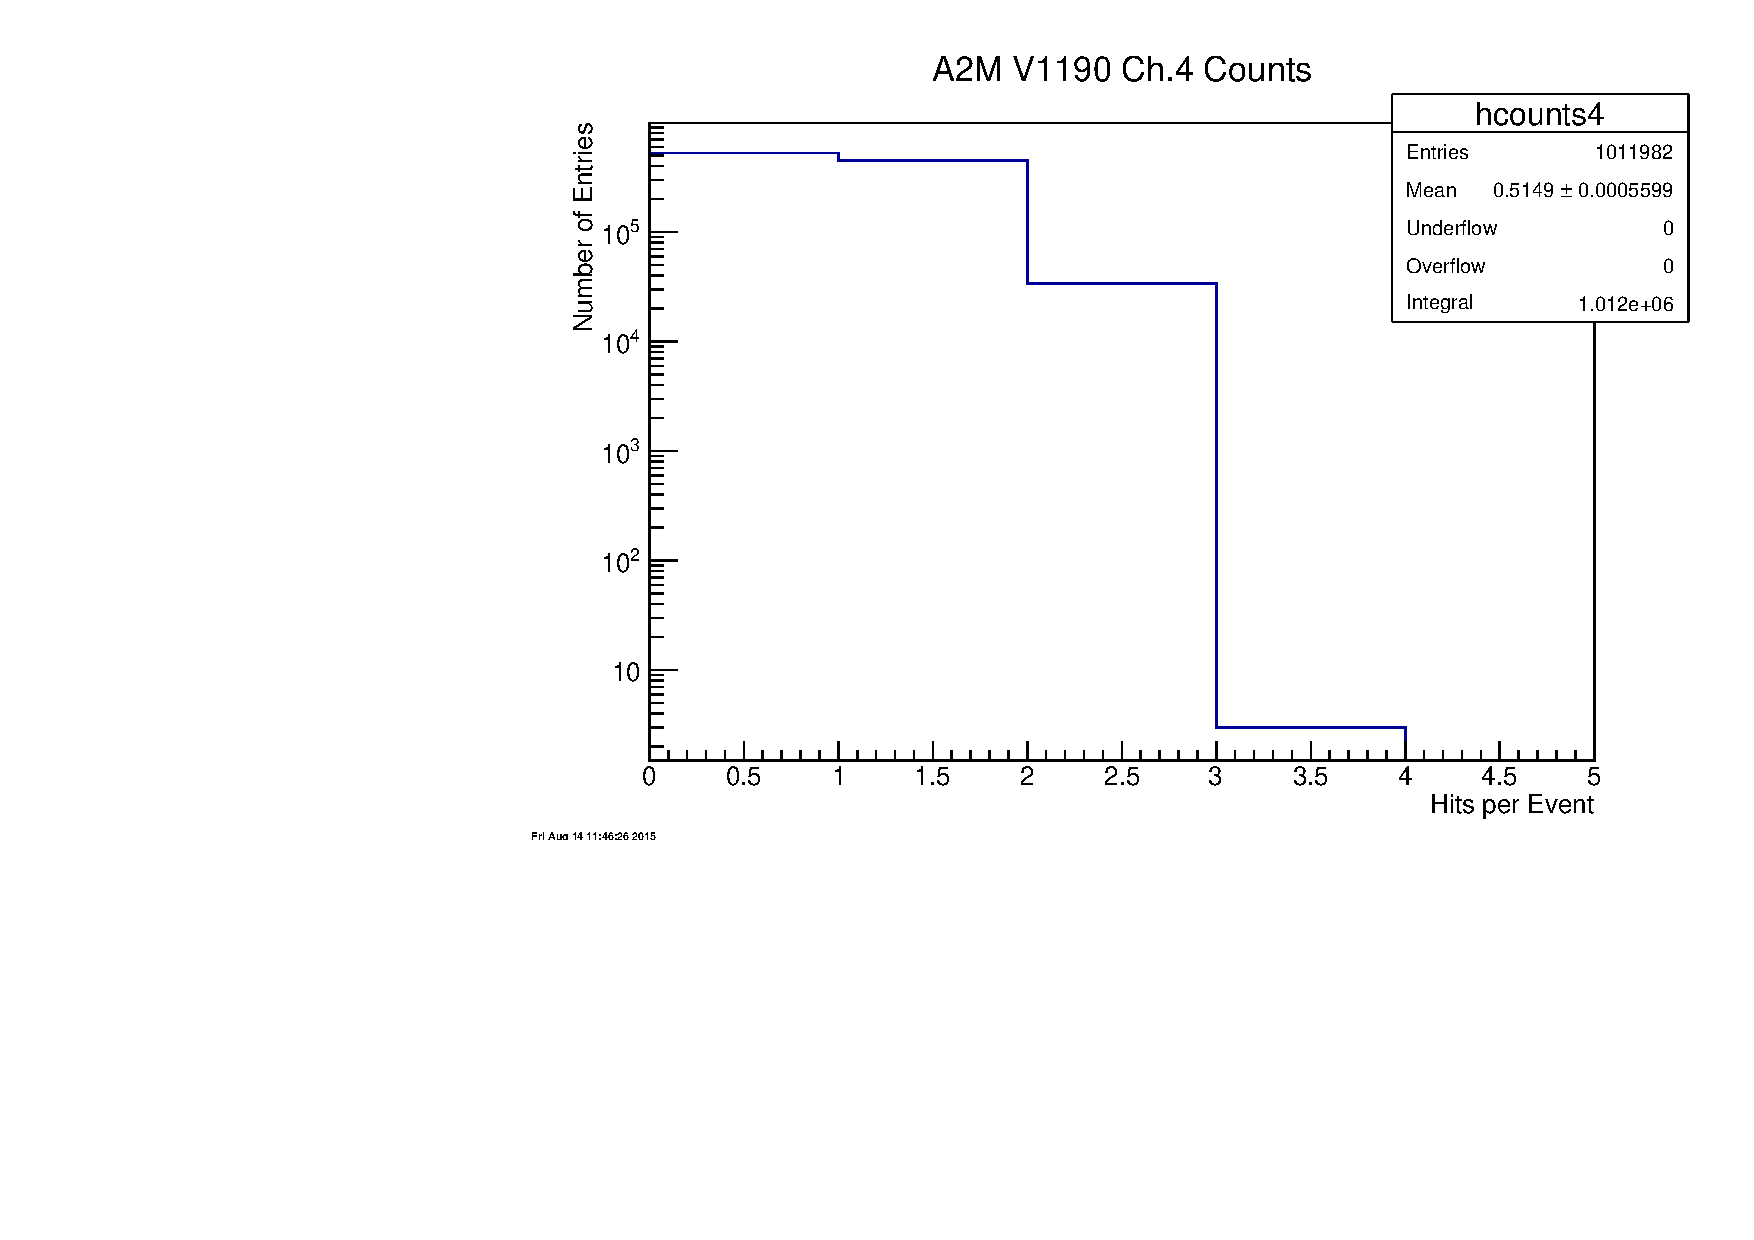
\includegraphics[width=0.4\textwidth,keepaspectratio]{run_606_hcounts4}\hspace{\fill}
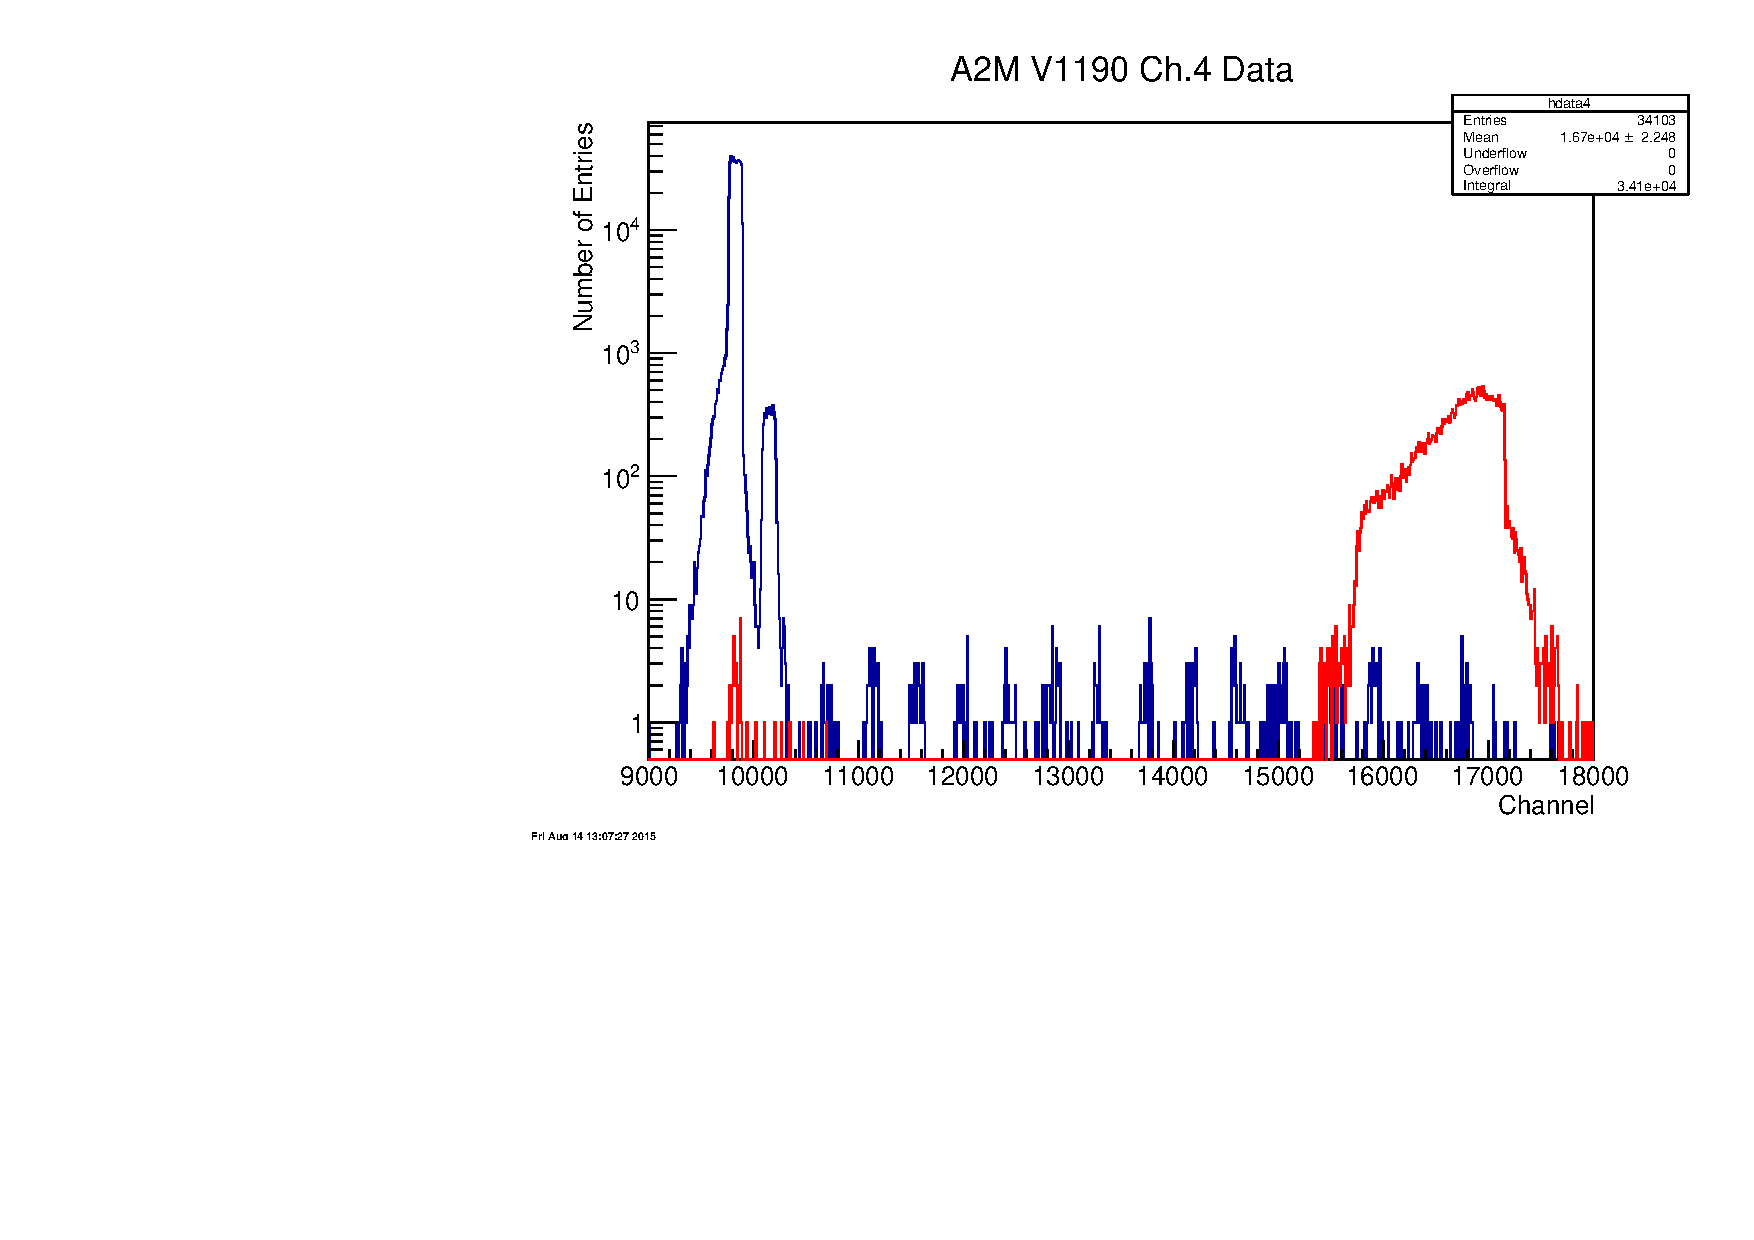
\includegraphics[width=0.4\textwidth,keepaspectratio]{run_606_hdata_1_2_zoom}\hspace{\fill}
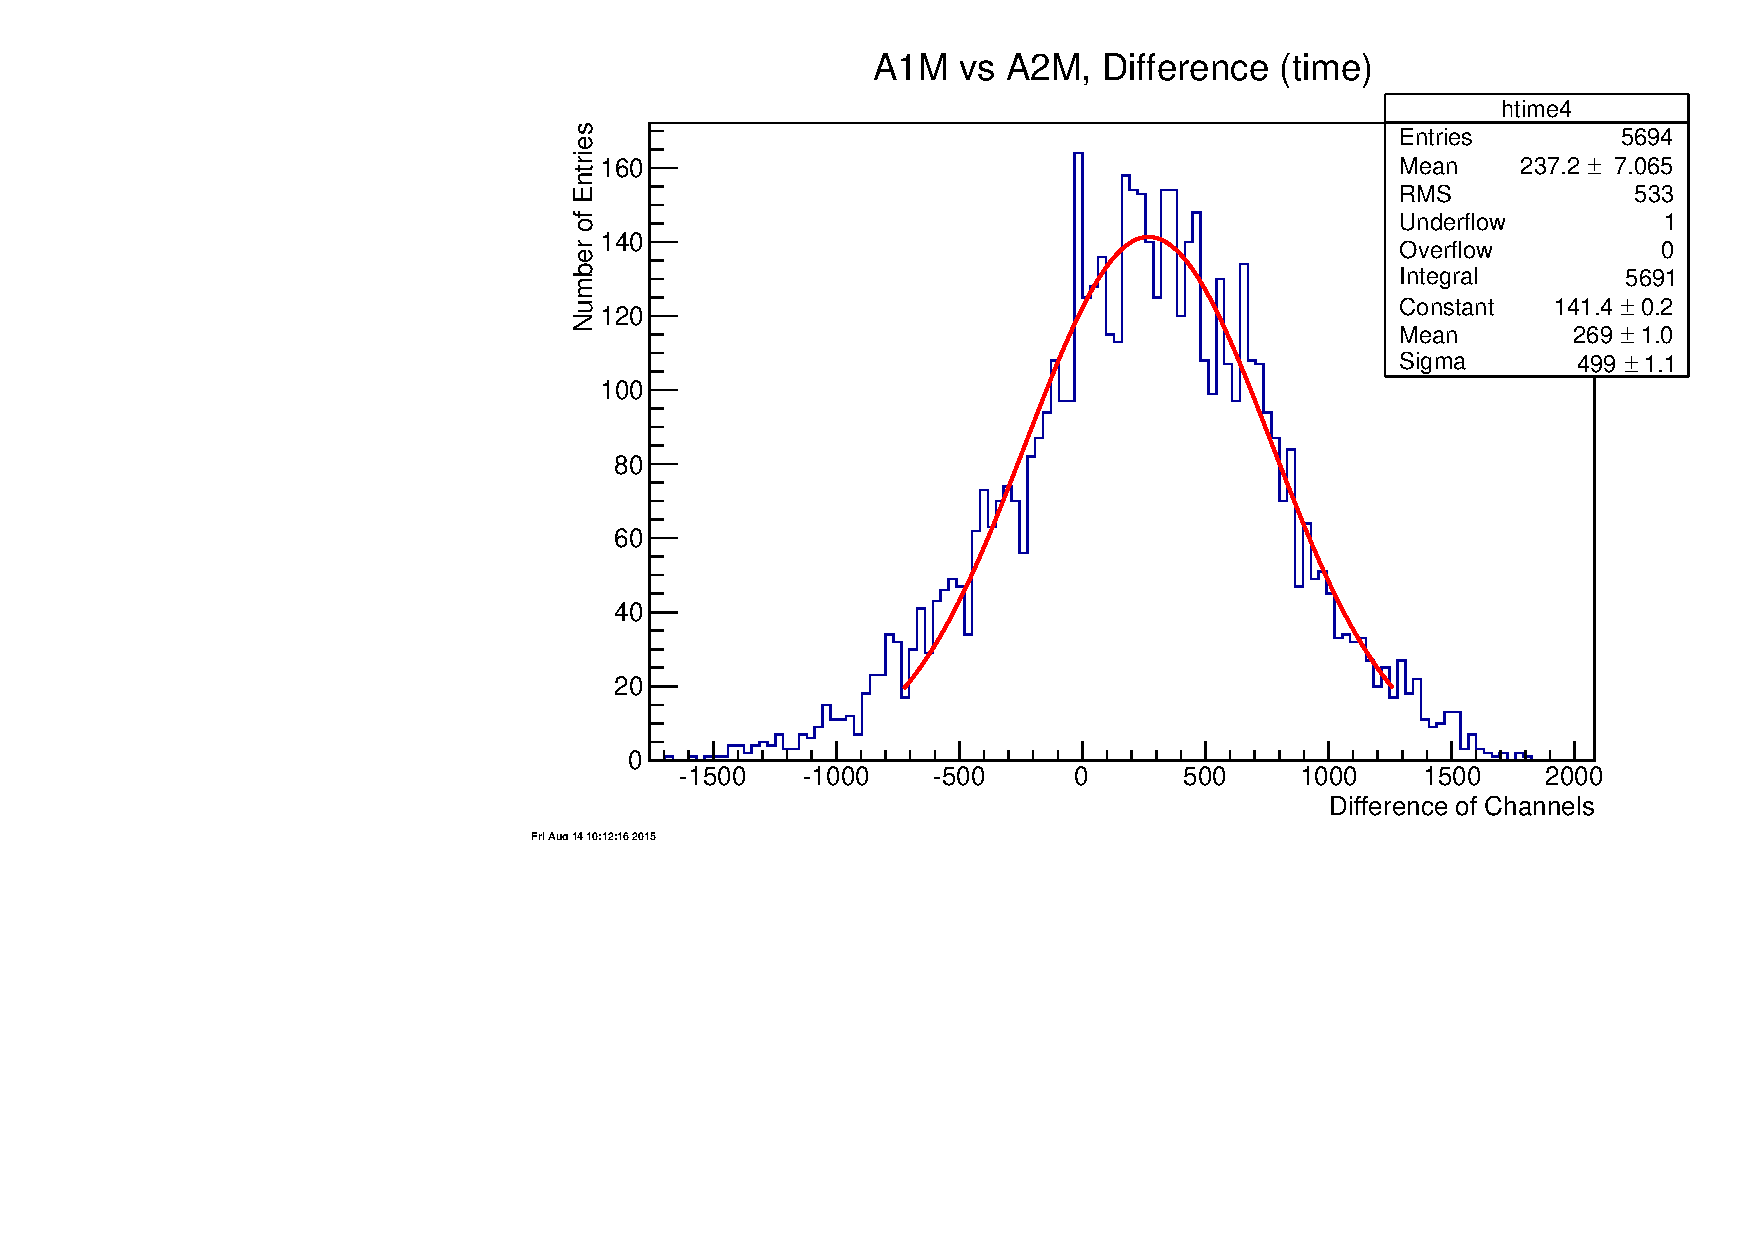
\includegraphics[width=0.4\textwidth,keepaspectratio]{run_606_htime4}\hspace{\fill}
}
\caption{(Left) Total multi-hit count spectrum from A2M. For $1\times10^6$ trigger events, 51.9\% of entries have no hits, 44.7\% of entries have exactly one hit, 3.4\% of entries have two hits, and 0.0\% of entries (3 events) have three hits. (Center) Raw data spectrum for A2M. Points corresponding to the first registered hit are shown in blue, points corresponding to the second hit are shown in red. (Right) Timing spectrum corresponding to events where both A1M and A2M have two hits; the difference of the second pair of hits is shown.
Compare with Fig.~\ref{diff_fit}.
The width of the peak 
%(499\,chan.~$\sigma$) 
is about $150\times$ that corresponding to the first pair of hits. 
}
\label{mhit}
\end{figure}

As of this writing, the multi-hit data for histogram sorting (\texttt{ana.cxx}) and tree sorting (\texttt{ana\_tree.cxx}) do not match. See Fig.~\ref{tree_comp} for details. The figure is generated with the following command.
\vsetroot
\begin{quote}
\begin{Verbatim}[firstnumber=0]
treecomp(0)
\end{Verbatim}
\end{quote}
\vsetnone
The cause of the mis-match is unknown is unknown.

\begin{figure}
\centering
\hspace{\fill}
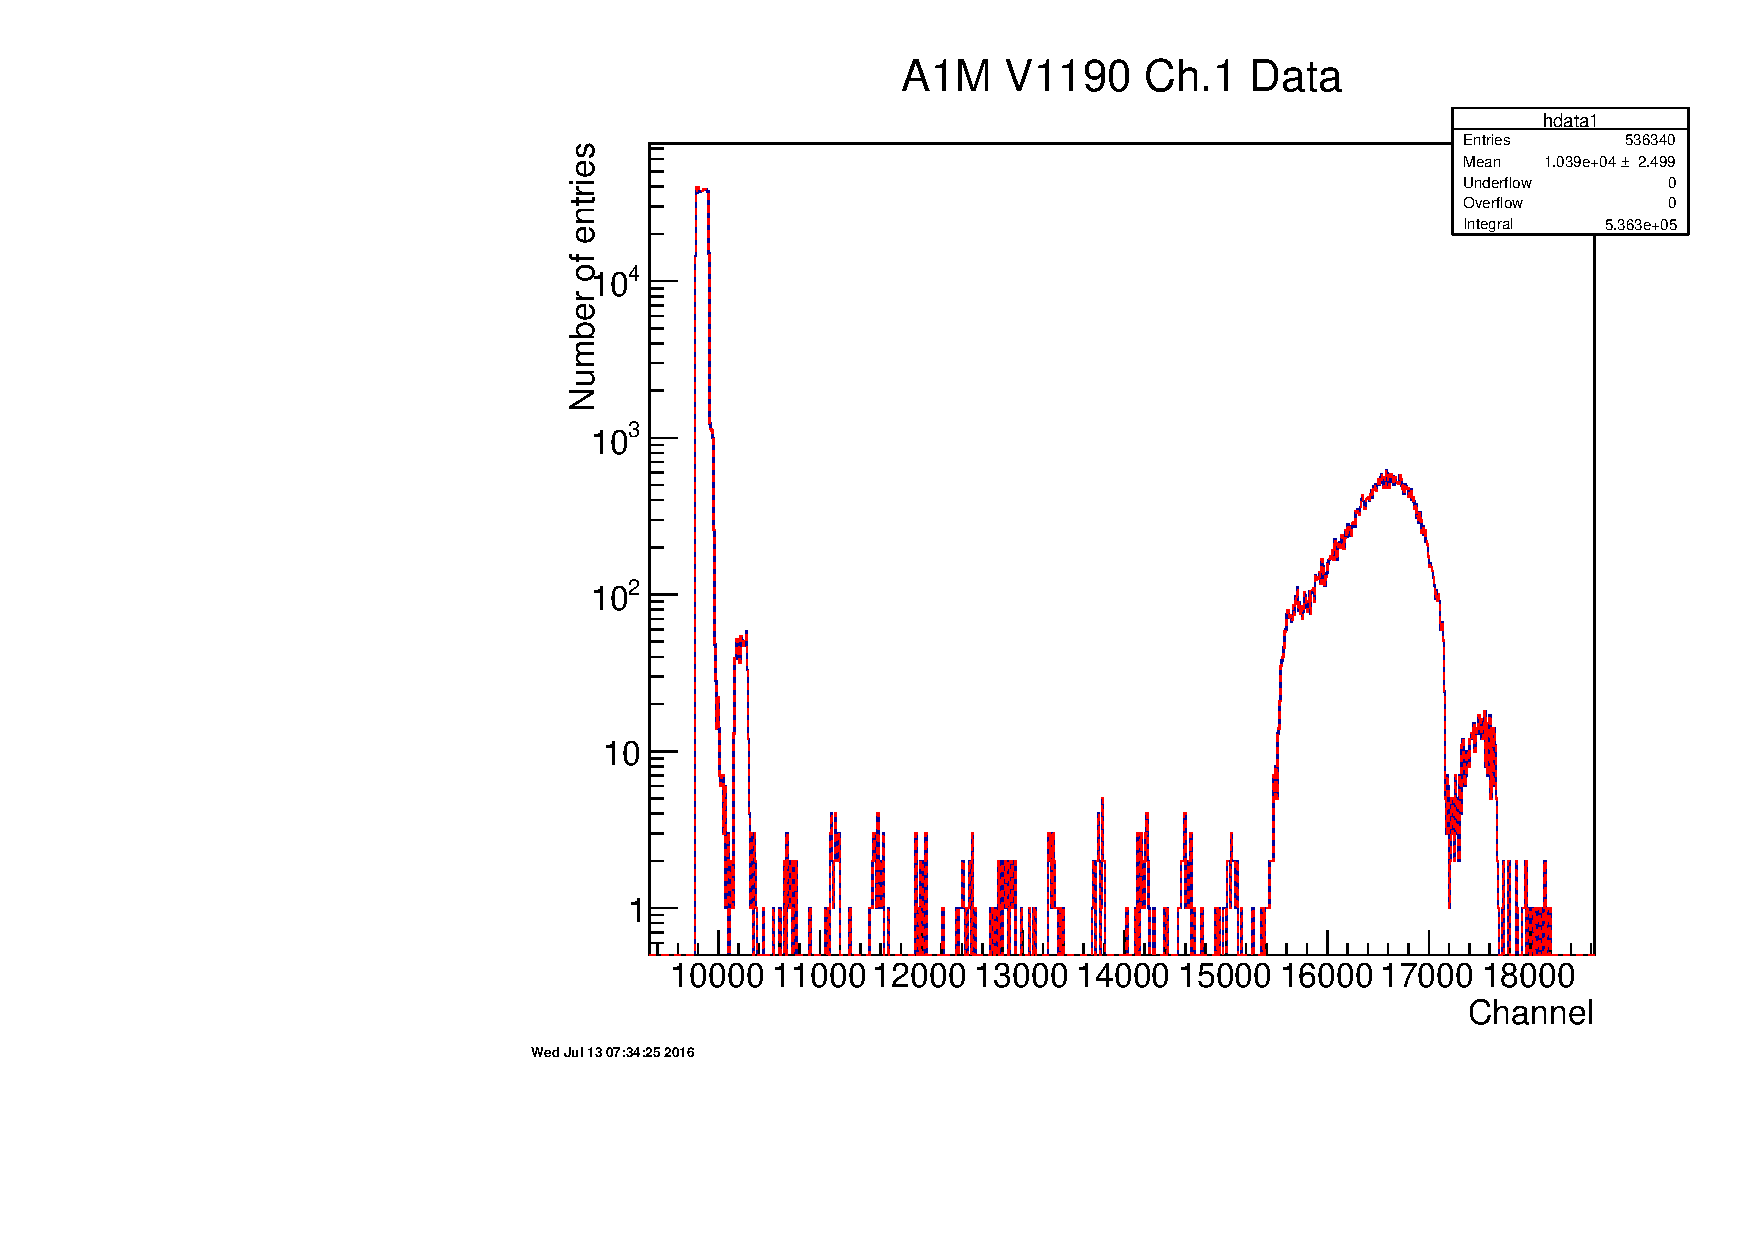
\includegraphics[width=0.48\textwidth, keepaspectratio]{run_606_treecomp1}\hspace{\fill}
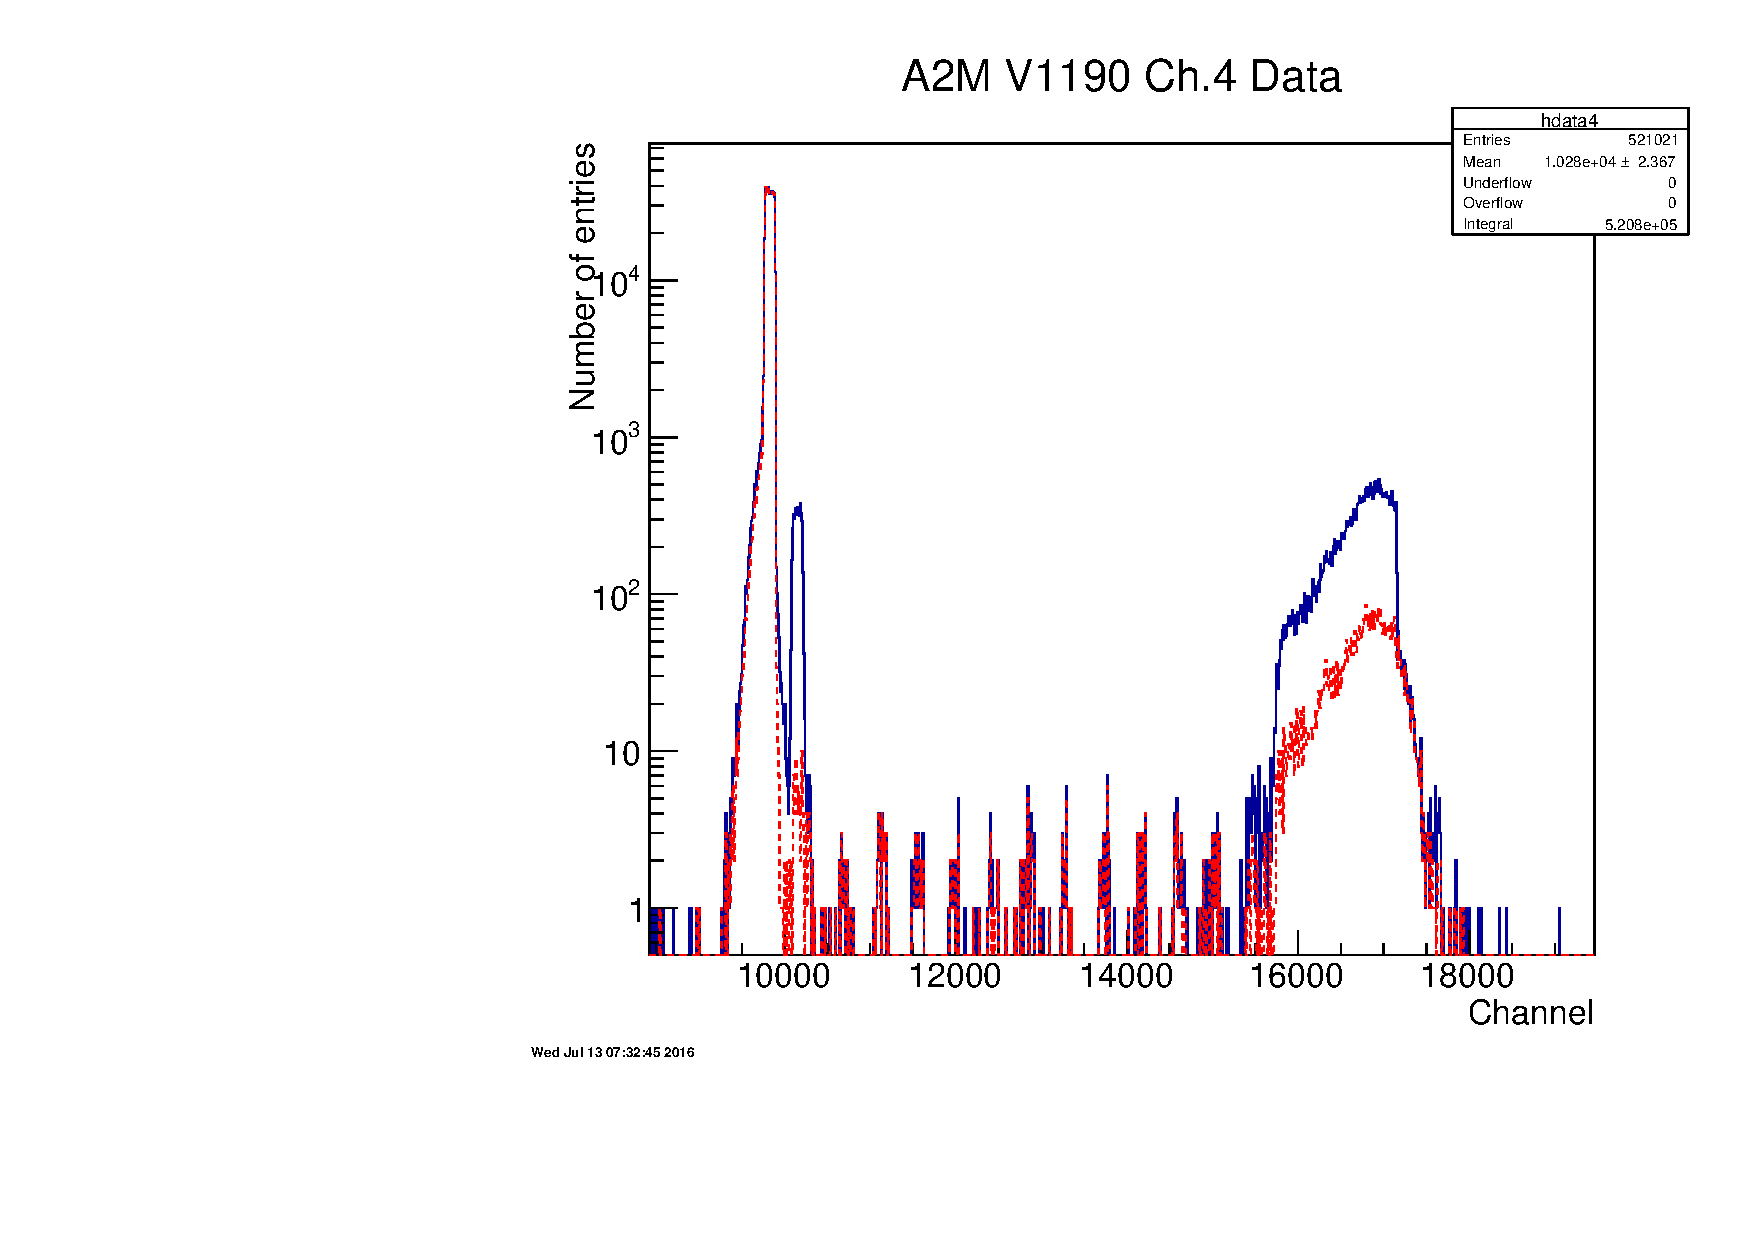
\includegraphics[width=0.48\textwidth, keepaspectratio]{run_606_treecomp4} \hspace{\fill}
\caption{Comparison of histogram sorting (blue, solid) and tree sorting (red, dashed) for anode A1M (left) and A2M (right). The two sorting methods agree for A1M, but disagree for A2M. The cause is unknown. In this example, the number of counts sorted into trees is 97\% of the counts sorted into histograms for A2M.}
\label{tree_comp}
\end{figure}


\subsection{Gain-matching}
\fussy
The first step in calibrating the detector data is to gain-matching each pair of detector signals.  Each of the 14 signals read out of the PGAC box is part of a pair.  Each cathode has a pair of signals (two pairs on each detector, four pairs in total) and each segment of the anode on each detector forms a pair (three in total).
\subsubsection{Anode Pairs}
\paragraph{Procedure}
\begin{sloppypar}
The two anodes measure the ionization from the same event in close proximity to each other ($\Delta z=36.80$\,mm).  Examining Fig.~\ref{lin_fit}\,(Left), one sees that the correlation between the anode timing signal pairs is sharply defined, linear, and the correlation coefficient is approximately equal to $+1$.  %Due to this approximate correlation,
%The timing signals from the two anodes is gain-matched such that the correlation coefficient is made 
This coefficient can be determined by plotting one of the signals in the pair against the other.  Using the \texttt{TProlile} class in ROOT, such a two-dimensional histogram may be fit with a one-dimensional function; in this case a linear polynomial.  This process is illustrated in Fig.~\ref{lin_fit}\,(Right). % for the anode signals.
This figure is generated using a command similar to the following.
\vsetroot
\begin{quote}
\begin{Verbatim}[firstnumber=0]
fitpfx("haaz4", 9700, 10100,9830,9950,1,0,0)
\end{Verbatim}
\end{quote}

\end{sloppypar}

\begin{figure}
\centering
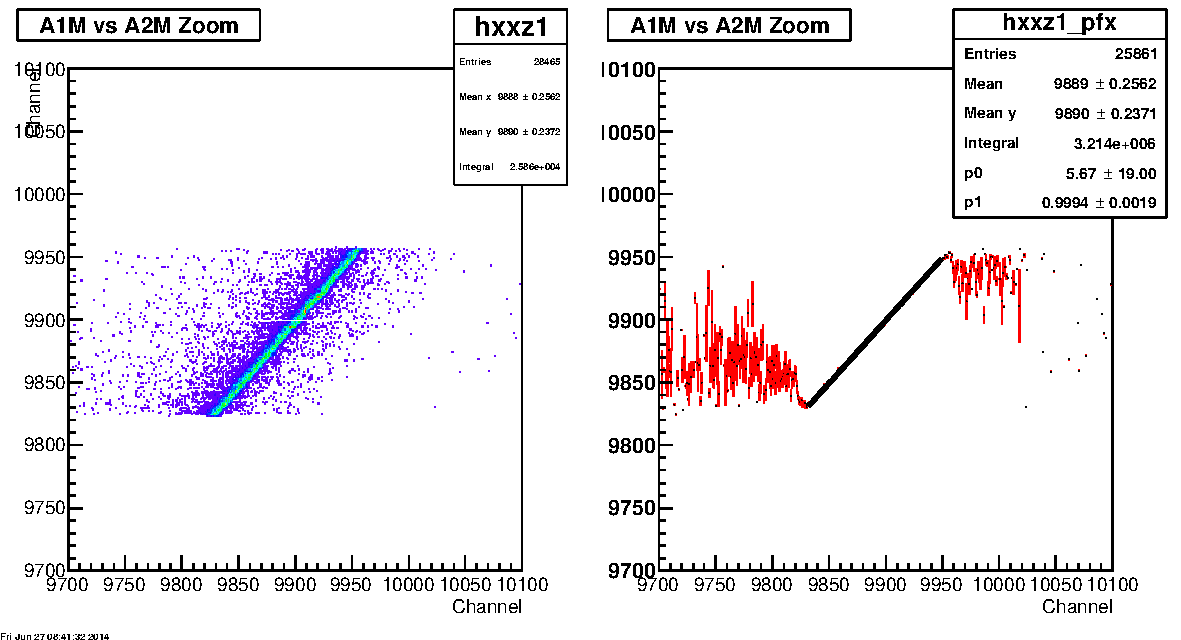
\includegraphics[width=\textwidth,keepaspectratio]{run00480_hxxz1_pfx}
\caption{Correlation plot of the anode signals.  (Left) A 2D histogram of A1M plotted against A2M is shown.  The histogram range is confined to the area of interest.  Note that the range of the signal A1M has sharp cutoffs because the anode signal from detector 1 is used to generate the trigger and is therefore self-gating. (Right) A 1D profile of the 2D histogram is fit with a linear function.}
\label{lin_fit}
\end{figure}

The quality of the linear fit verifies that the pairs of anode signals are linearly correlated.  Higher-order corrections are not necessary.  With such sharply correlated data, the slope of the fit %provides 
is closely related to the the correlation coefficient.  The goal of gain-matching the anode pairs is to minimize the width of the distribution of difference the signals.  When this is accomplished, the correlation coefficient is approximately equal to $+1$. %, thus gain-matching the signals,

\paragraph{Method}
To first order, the gain-matching is accomplished by scaling the signal plotted as the ordinate ($y$-axis) by the slope of the fit.  For the anode pairs, the signal from detector 1 is plotted on the $y$-axis.  The gain-matching technique is implemented for the anodes using the following block of code. The calibration parameters are read in from a file at the start of the analysis.  The calibration files are named for the run number, such as \texttt{run\_480.cal}.
\vspace{0.5\baselineskip}
\par\noindent
\begin{minipage}{\linewidth}
  \singlespace
\begin{lstlisting}[caption={Gain-match andode. Here the uncalibrated signal \texttt{a[i][0]} is scaled in two steps.   First, with scaling parameter derived from the slope, \texttt{hxxcal[i][1]}; and then with an offset parameter \texttt{hxxcal[i][0]}.
  The output is saved in \texttt{a[i][1]}.
The fit parameters of each correlation plot are stored in the array \texttt{hxxcal[i][j]}.  The index \texttt{[i]} runs from 0--3 for each of the 3 signal pairs and the index \texttt{[j]} runs from 0--1 for the linear fit parameters; 0 for offset, 1 for slope.}]
if(docal) { 
  a[i][1]=a[i][0]/hxxcal[i][1];	 
  a[i][1]-=hxxcal[i][0];
}
\end{lstlisting}
%a1/=hxxcal[i][1];	 
%a1-=hxxcal[i][0];
%\vspace{-1\baselineskip}
\end{minipage}


The gain-matching can be fine-tuned by adjusting the scaling parameter to minimize the  difference of the anode signal pairs.  In other words, the scale parameter is adjusted to minimize the measured width $\sigma$ of a Gaussian fit of the distribution.  This procedure is illustrated in Fig.~\ref{diff_fit}.  When the %With a
 correlation coefficient identically equal to $+1$, the difference of the anode signals should be constant; in this case equal to zero. %In a similar manner, the 
 Accordingly, the offset parameter \texttt{hxxcal[i][0]} is fine-tuned to adjust the mean of the difference to zero. Typical calibration parameters are shown in Table~\ref{anode-calib}.
 
\begin{table}[ht]
\centering  
\begin{tabular}{c..}
\hline
\multicolumn{1}{c}{Pair}& \multicolumn{1}{c}{Offset}& \multicolumn{1}{c}{Slope} \\
\multicolumn{1}{c}{\texttt{i}}&\multicolumn{1}{c}{\texttt{hxxcal[i][0]}}&\multicolumn{1}{c}{\texttt{hxxcal[i][1]}}\\ \hline \hline
 0 & 16.652191 & 0.999918377\\
 1 & 11.5593   & 0.999854499\\
 2 & 3.80868   & 0.999757652\\
 \hline 
\end{tabular}
\caption{Typical calibration constants for each of the three  anode pairs (\texttt{i}). Parameters are given for run 606. The average value of \texttt{hxxcal[i][1]} is different from 1 by an average value of 2/10,000. 
%can be correlated with each of the three anode segment pairs (\texttt{k}); twelve combinations in total. The index runs from 0--11 and is defined by $(\texttt{i}-3)\times 3 + \texttt{k}$.
}
\label{anode-calib}
\end{table}
 
\begin{figure}[ht]
\centering
\hspace{\fill}
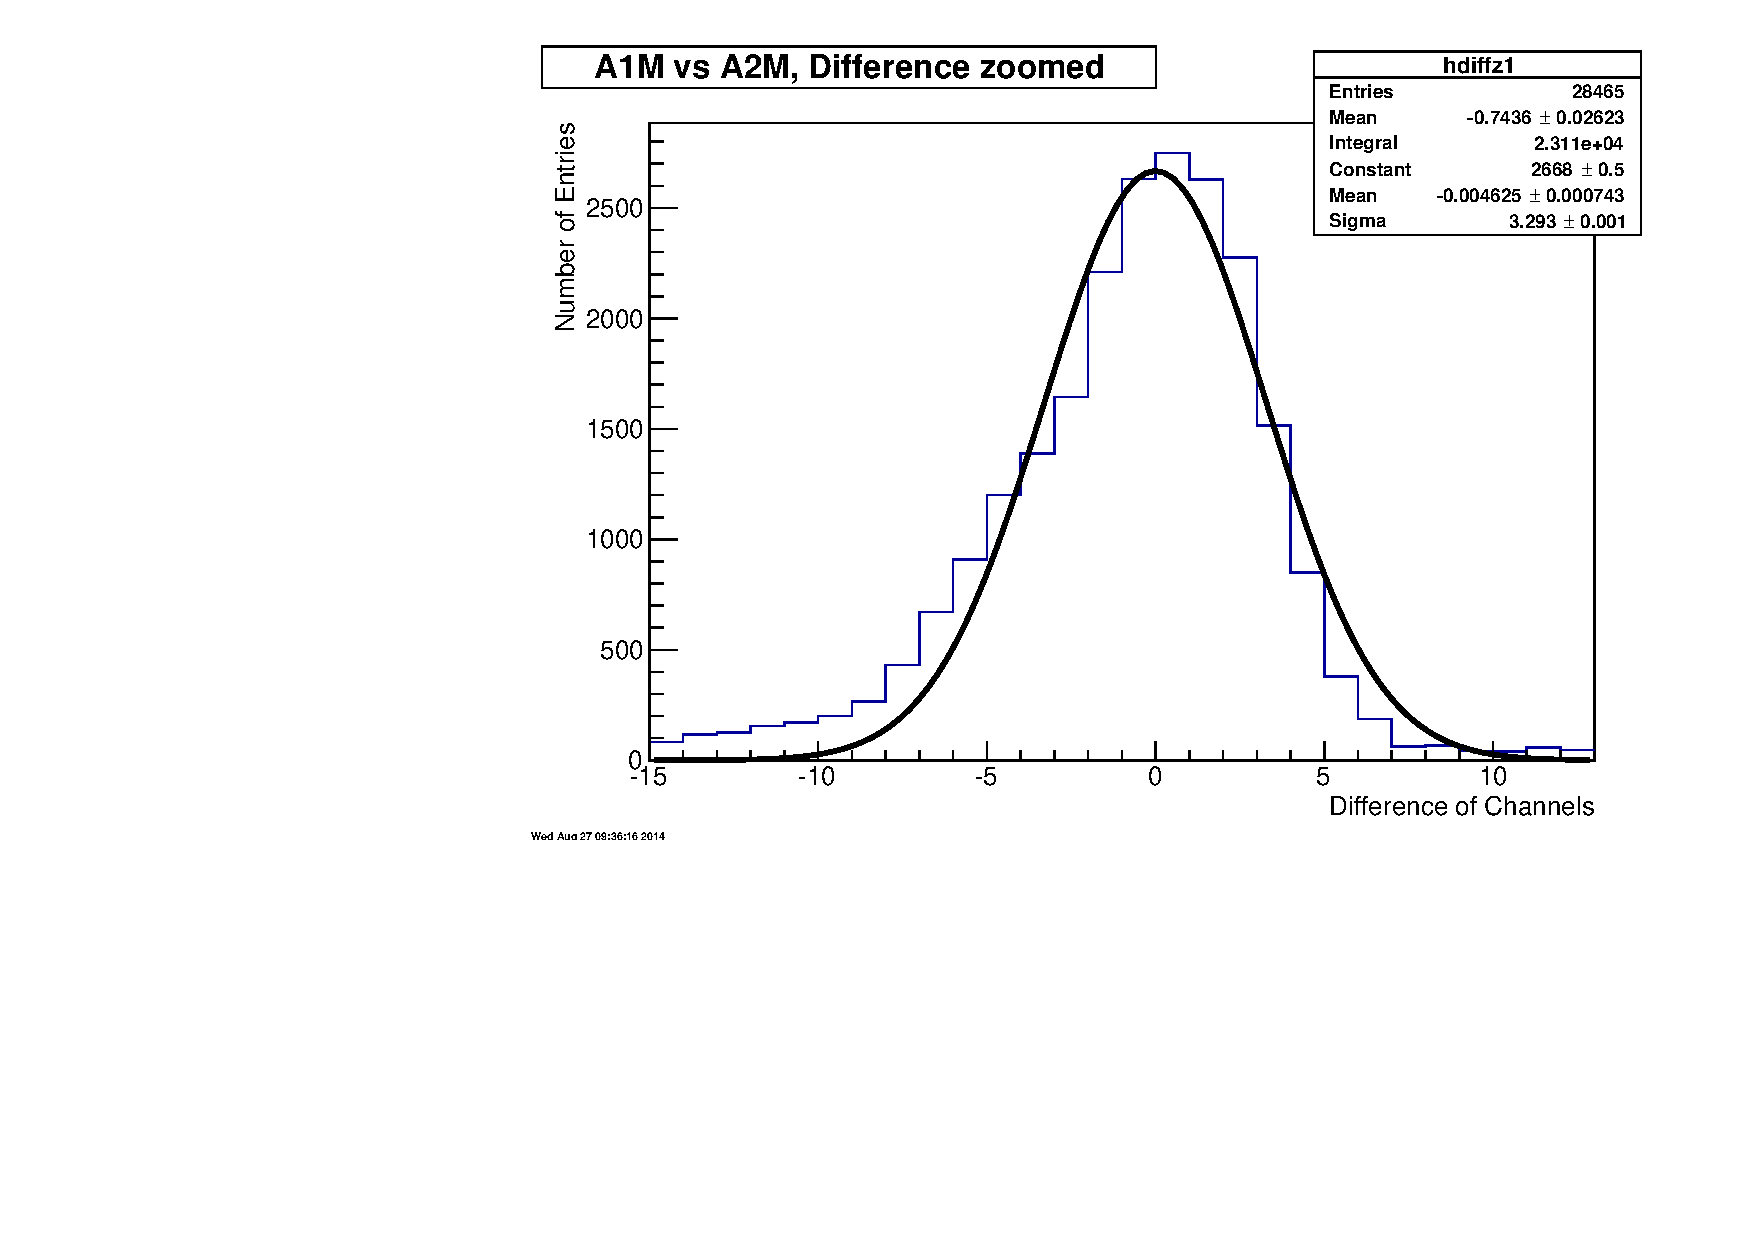
\includegraphics[width=0.48\textwidth,keepaspectratio]{run_480_hdiffz1_fit}\hspace{\fill}
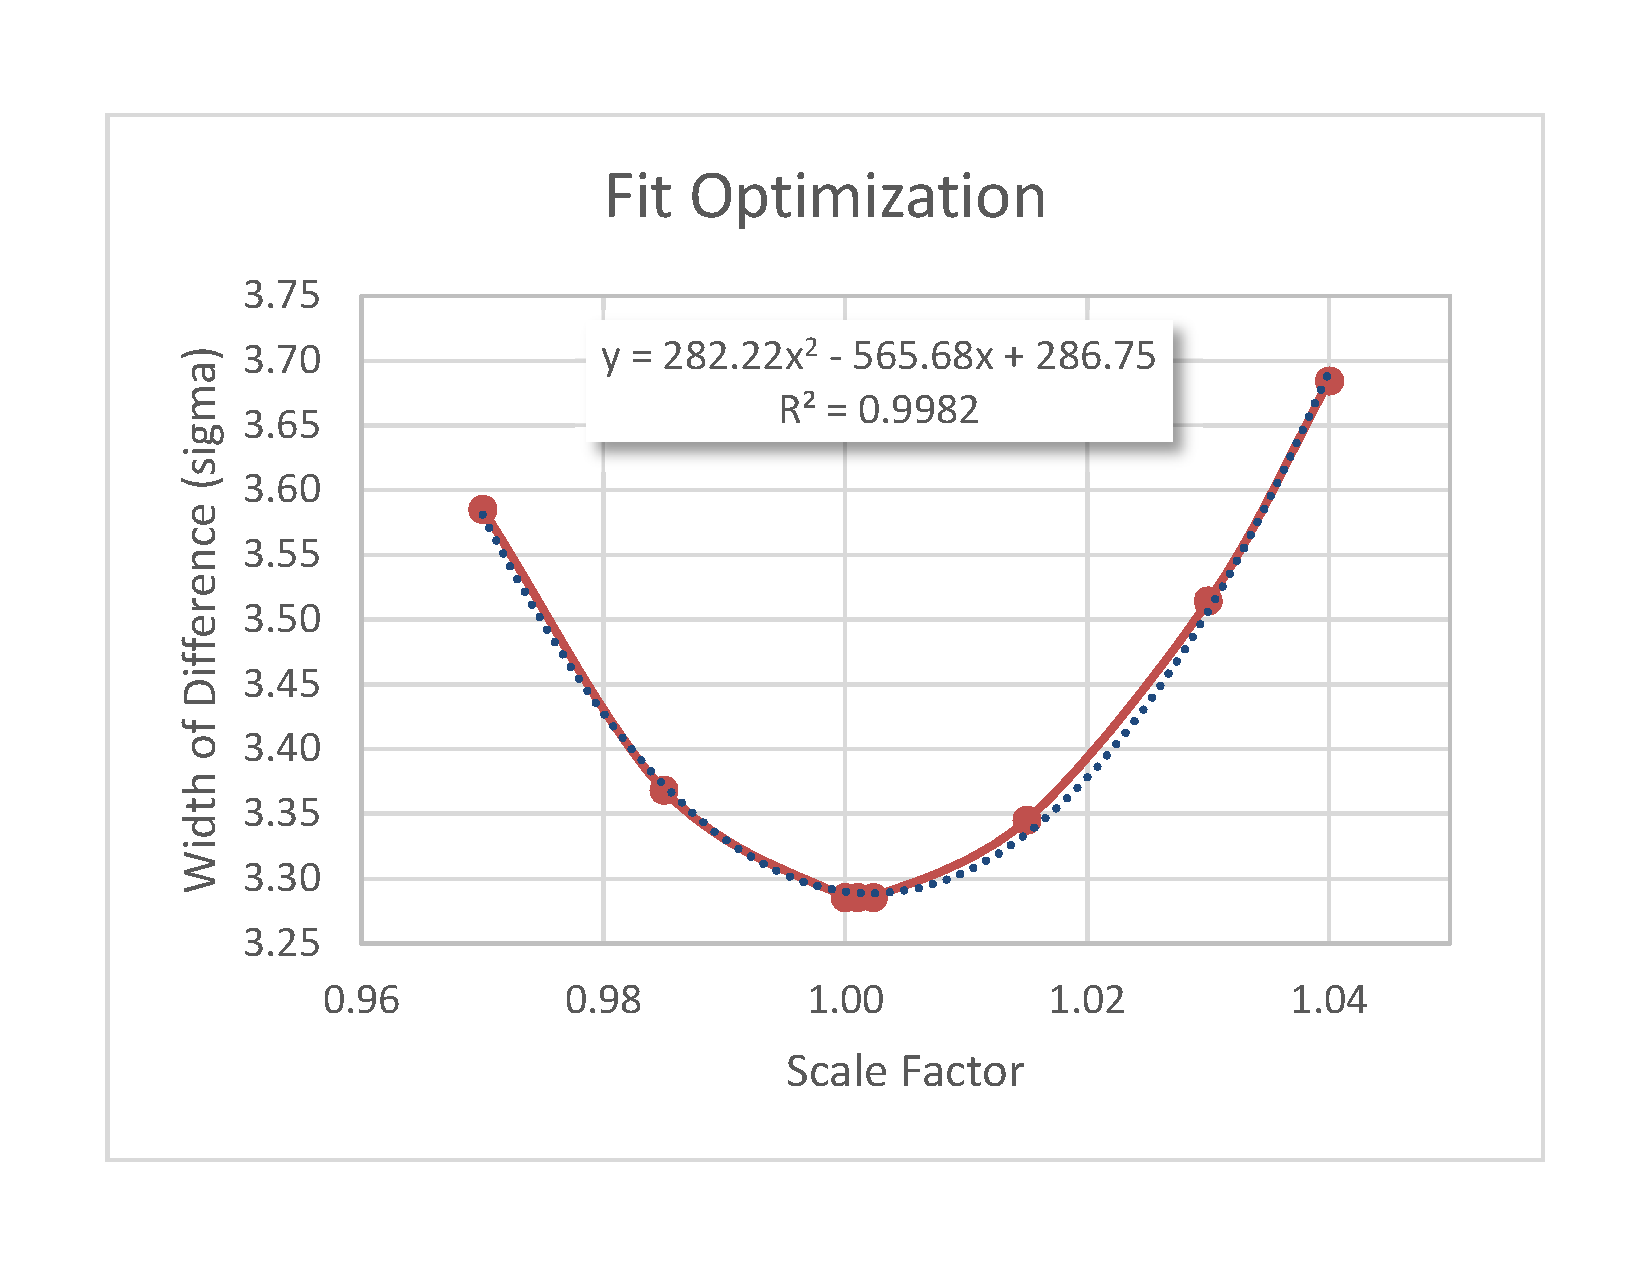
\includegraphics[width=0.48\textwidth, keepaspectratio]{hdiffz1} \hspace{\fill}
\caption{(Left) The %sum of 
difference of the anode signals are plotted and fit with a gaussian function %with X1R
after one of the positions has been scaled by %with a given 
the value of the parameter \texttt{hxxcal[1][1]}.  (Right) The value of the sigma of the gaussian fits is plotted against the scaling factor  \texttt{hxxcal[1][1]}.  The distribution is then fit with a quadratic function to calculate the best fit, in this case $1.00231$.}
\label{diff_fit}
\end{figure}

\subsubsection{Cathode Pairs}
\paragraph{Procedure}
Each pair of position signals from the cathodes are also linearly correlated.  The origin of this correlation is derived from the physical characteristics of the detector.  First, as discussed in \S\,\ref{position_description}, the delay applied to each position signal is directly-proportional to the distance of the incident ionization from each end of the detector.  Explicitly, this means that events closer to the edge of the detector have a smaller delay. Second, the sum of the delays for each position signal pair is constant (because the length of the detector is constant).  Therefore, the correlation coefficient between cathode pairs should be identically equal to $-1$. A correlation plot for a pair of position signals is shown in the appendix in Fig.~\ref{reflect}\,(Left). As is the case with the anode signals, the cathode signals can be gain-matched by scaling one of the signals by a linear offset.
\paragraph{Method}
The gain-matching technique is implemented for the cathodes using the following block of code.
%\pangram{100}
\vspace{0.5\baselineskip}
\par\noindent
\begin{minipage}{\linewidth}
  \singlespace
\begin{lstlisting}[caption={The index \texttt{i} runs over 3--6 for each cathode pair. Here \texttt{xn[i-3][0]} refers to the (uncalibrated) ``near'' position signal and \texttt{xf[i-3][0]} refers to the ``far'' position signal.  These labels correspond to those given in Table~\ref{TDC_signals} and are defined from the perspective of the beam.   The nested \texttt{if} statement is used so that neither signal is compressed; one of the signals is expanded to set the correlation coefficient to $-1$.},label=cathode_scaling]
if(docal) {
  if(hxxcal[i][1]<-1.) {
    xn[i-3][1]=xn[i-3][0]*(-hxxcal[i][1]);
    xf[i-3][1]=xf[i-3][0];
  }
  else {
    xn[i-3][1]=xn[i-3][0]; 
    xf[i-3][1]=xf[i-3][0]*(-1./hxxcal[i][1]);
  }
}
\end{lstlisting}
%   xn=(-hxxcal[i][1])*xn;
%  }
%  else{
%    xf=(-1./hxxcal[i][1])*xf;
%  }
%}
%\vspace{-1\baselineskip}
\end{minipage}

%\subsubsection{Verification}
As previously stated, the sum of the position signals should be constant.
% and the difference of the anode signals should be constant.
In a manner similar to that used with the anode signals, %Therefore, 
the scale factor can be adjusted to minimize the width of the sum of the position signals. % and the difference of the anode signals. 
 This procedure is illustrated in Fig.~\ref{sum_fit}. 
\begin{figure}
\centering
\hspace{\fill}
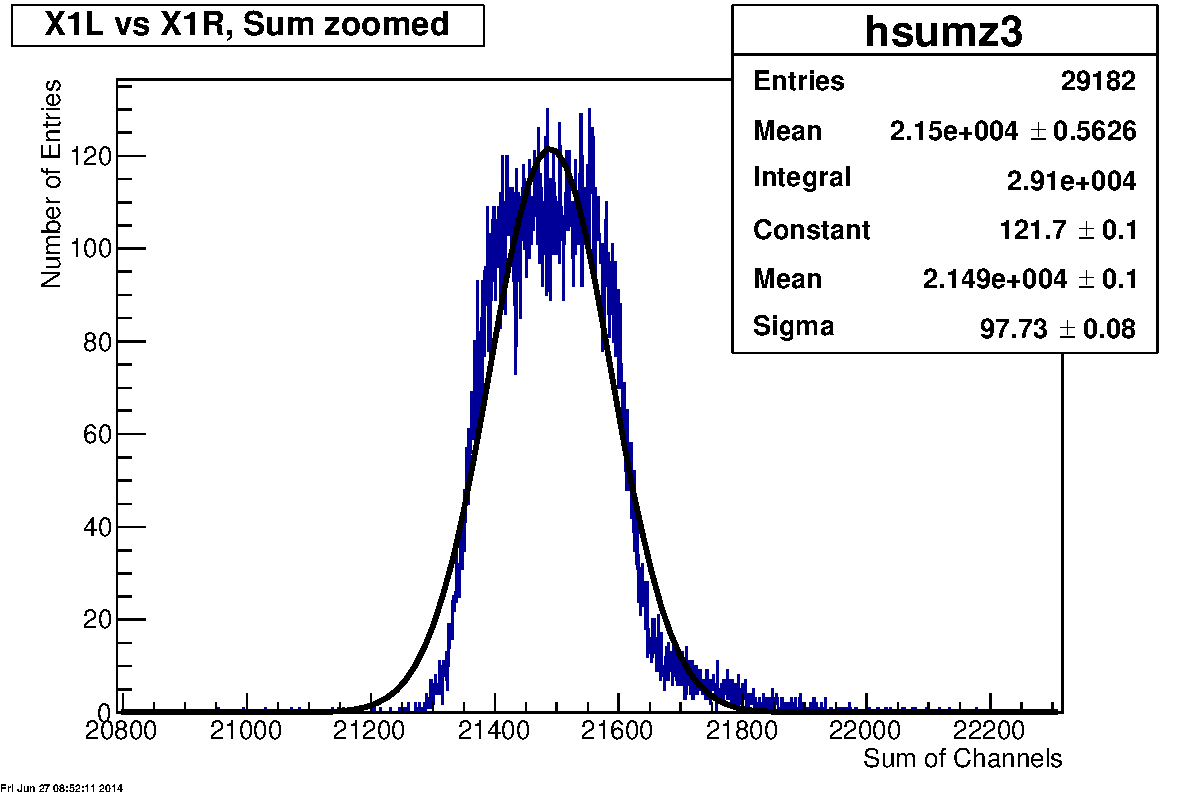
\includegraphics[width=0.48\textwidth,keepaspectratio]{run00480_hsumz3}\hspace{\fill}
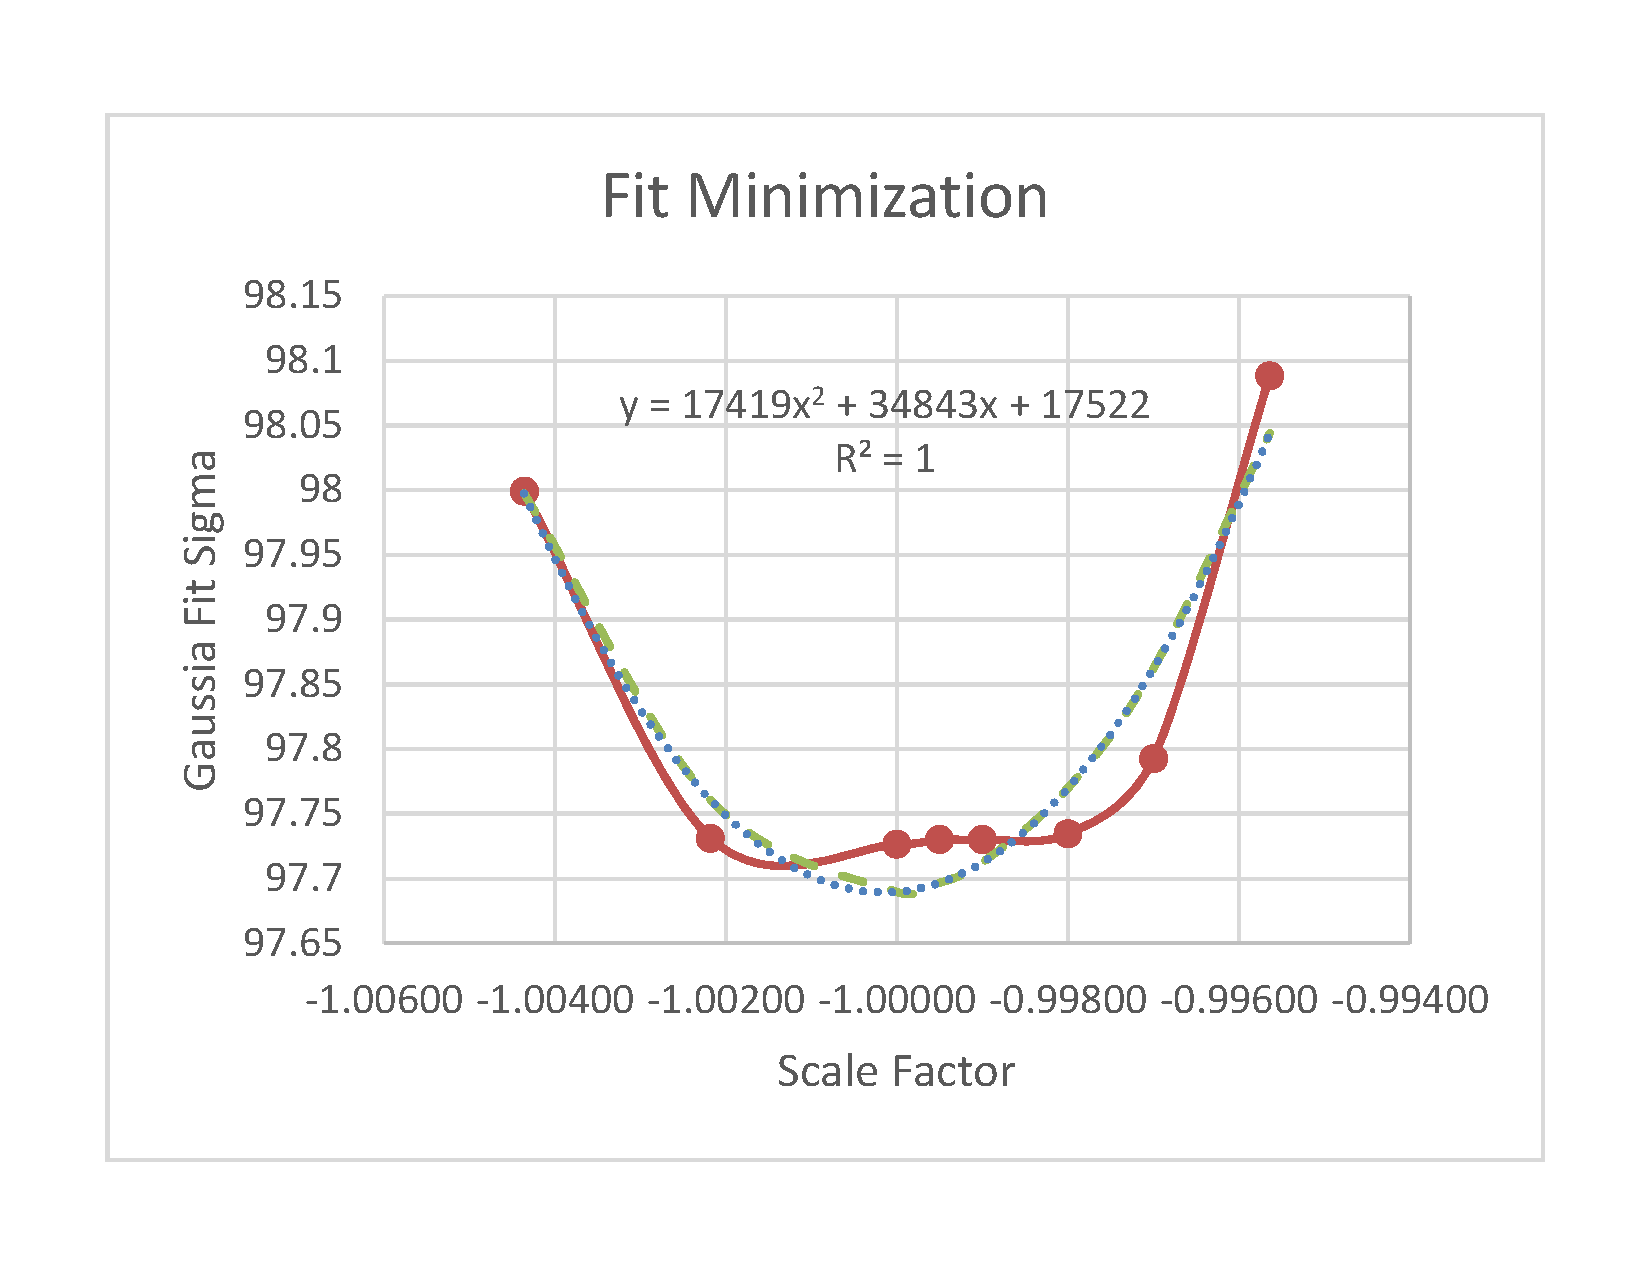
\includegraphics[width=0.48\textwidth, keepaspectratio]{hsumz3_fit} \hspace{\fill}
\caption{(Left) The %sum of 
position signals X1L and X1R are summed and fit with a gaussian function %with X1R
after one of the positions has been scaled by %with a given 
the value of the parameter \texttt{hxxcal[3][1]}.  (Right) The value of the sigma of the gaussian fits is plotted against the scaling factor  \texttt{hxxcal[3][1]}.  The distribution is then fit with a quadratic function to calculate the best fit, in this case $-1.00015$.}
\label{sum_fit}
\end{figure}
In this example, the width of the sum of the position signals X1L and X1R was measured for several values of the scaling parameter \texttt{hxxcal[3][1]}.  The resulting distribution was fit with a quadratic function to locate the value of \texttt{hxxcal[3][1]} that corresponds to the minimum width of the sum. Table~\ref{cathode-calib} shows some typical calibration values.

\begin{table}[ht!]
\centering  
\begin{tabular}{c..}
\hline
\multicolumn{1}{c}{Pair}& \multicolumn{1}{c}{Offset}& \multicolumn{1}{c}{Slope} \\
\multicolumn{1}{c}{\texttt{i}}&\multicolumn{1}{c}{\texttt{hxxcal[i][0]}}&\multicolumn{1}{c}{\texttt{hxxcal[i][1]}}\\ \hline \hline
 3 & 0 & -1.00152409\\
 4 & 0 & -1.002232225\\
 5 & 0 & -1.000613607\\
 6 & 0 & -0.995592661\\
 \hline 
\end{tabular}
\caption{Typical calibration constants for each of the 4 cathode pairs (\texttt{i}). Given for run 480. The average value of \texttt{hxxcal[i][1]} is different from -1 by an average value of 2/1,000. 
Note that the offset variable is not used.
%can be correlated with each of the three anode segment pairs (\texttt{k}); twelve combinations in total. The index runs from 0--11 and is defined by $(\texttt{i}-3)\times 3 + \texttt{k}$.
}
\label{cathode-calib}
\end{table}

%\subsubsection{Anode Segments}
\subsubsection{Anode-Cathode}
\paragraph{Procedure}
Comparing the gain-matching procedure for the anodes and cathodes, two particular features are evident. First, the width of the correlations  for the cathodes appears to be much broader than that of the anodes (compare Fig.~\ref{lin_fit}\,(Left) with Fig.~\ref{reflect}\,(Left) in the Appendix).  Second, the width of the difference of the anode signals is more sharply defined and responds to scaling in a more predicable manner than the sum of the cathode signals (compare Fig.~\ref{diff_fit} with Fig.~\ref{sum_fit}).  The origin of this discrepancy can be revealed by comparing the cathode pairs with their corresponding anode. 

Each cathode pair can be correlated to an anode signal.  There are four cathode pairs in total corresponding to the two position pairs are each of the two detectors. There are three anodes %pairs
 corresponding to the three %anode 
 segments on each detector. This configuration yields twelve possible combinations.  The combinations are summarized in Table.~\ref{position-andode}.  For example, the sum of the Y2 signals are plotted against the anode signal of detector 2 in Fig.~\ref{hsa}.  By inspection, it can be seen that the sum of the position signals varies with the anode signal.  However, as discussed, the sum of the cathode signals should be constant.
\begin{table}[ht!]%
\centering  
\begin{tabular}{ccccc}
%\begin{tabulary}{1.0\textwidth}{ccccc} 
\hline
\multicolumn{1}{c}{Index} & \multicolumn{1}{c}{Pair}& \multicolumn{1}{c}{Segment}& Position & Anode \\
&\multicolumn{1}{c}{\texttt{i}}&\multicolumn{1}{c}{\texttt{k}}\\ \hline \hline
 0 & 3 & 0 & \texttt{X1} & \texttt{A1B} \\
 1 & 3 & 1 & \texttt{X1} & \texttt{A1M} \\
 2 & 3 & 2 & \texttt{X1} & \texttt{A1T} \\
 3 & 4 & 0 & \texttt{Y1} & \texttt{A1B} \\
 4 & 4 & 1 & \texttt{Y1} & \texttt{A1M} \\
 5 & 4 & 2 & \texttt{Y1} & \texttt{A1T} \\
 6 & 5 & 0 & \texttt{X2} & \texttt{A2B} \\
 7 & 5 & 1 & \texttt{X2} & \texttt{A2M} \\
 8 & 5 & 2 & \texttt{X2} & \texttt{A2T} \\
 9 & 6 & 0 & \texttt{Y2} & \texttt{A2B} \\
10 & 6 & 1 & \texttt{Y2} & \texttt{A2M} \\
11 & 6 & 2 & \texttt{Y2} & \texttt{A2T} \\
 \hline 
\end{tabular}
%\end{tabulary}
\caption{Each of the four position pairs (\texttt{i}) can be correlated with each of the three anode segment pairs (\texttt{k}); twelve combinations in total. The index runs from 0--11 and is defined by $(\texttt{i}-3)\times 3 + \texttt{k}$.}
\label{position-andode}
\end{table}
\begin{figure}[ht]
\centering
\hspace{\fill}
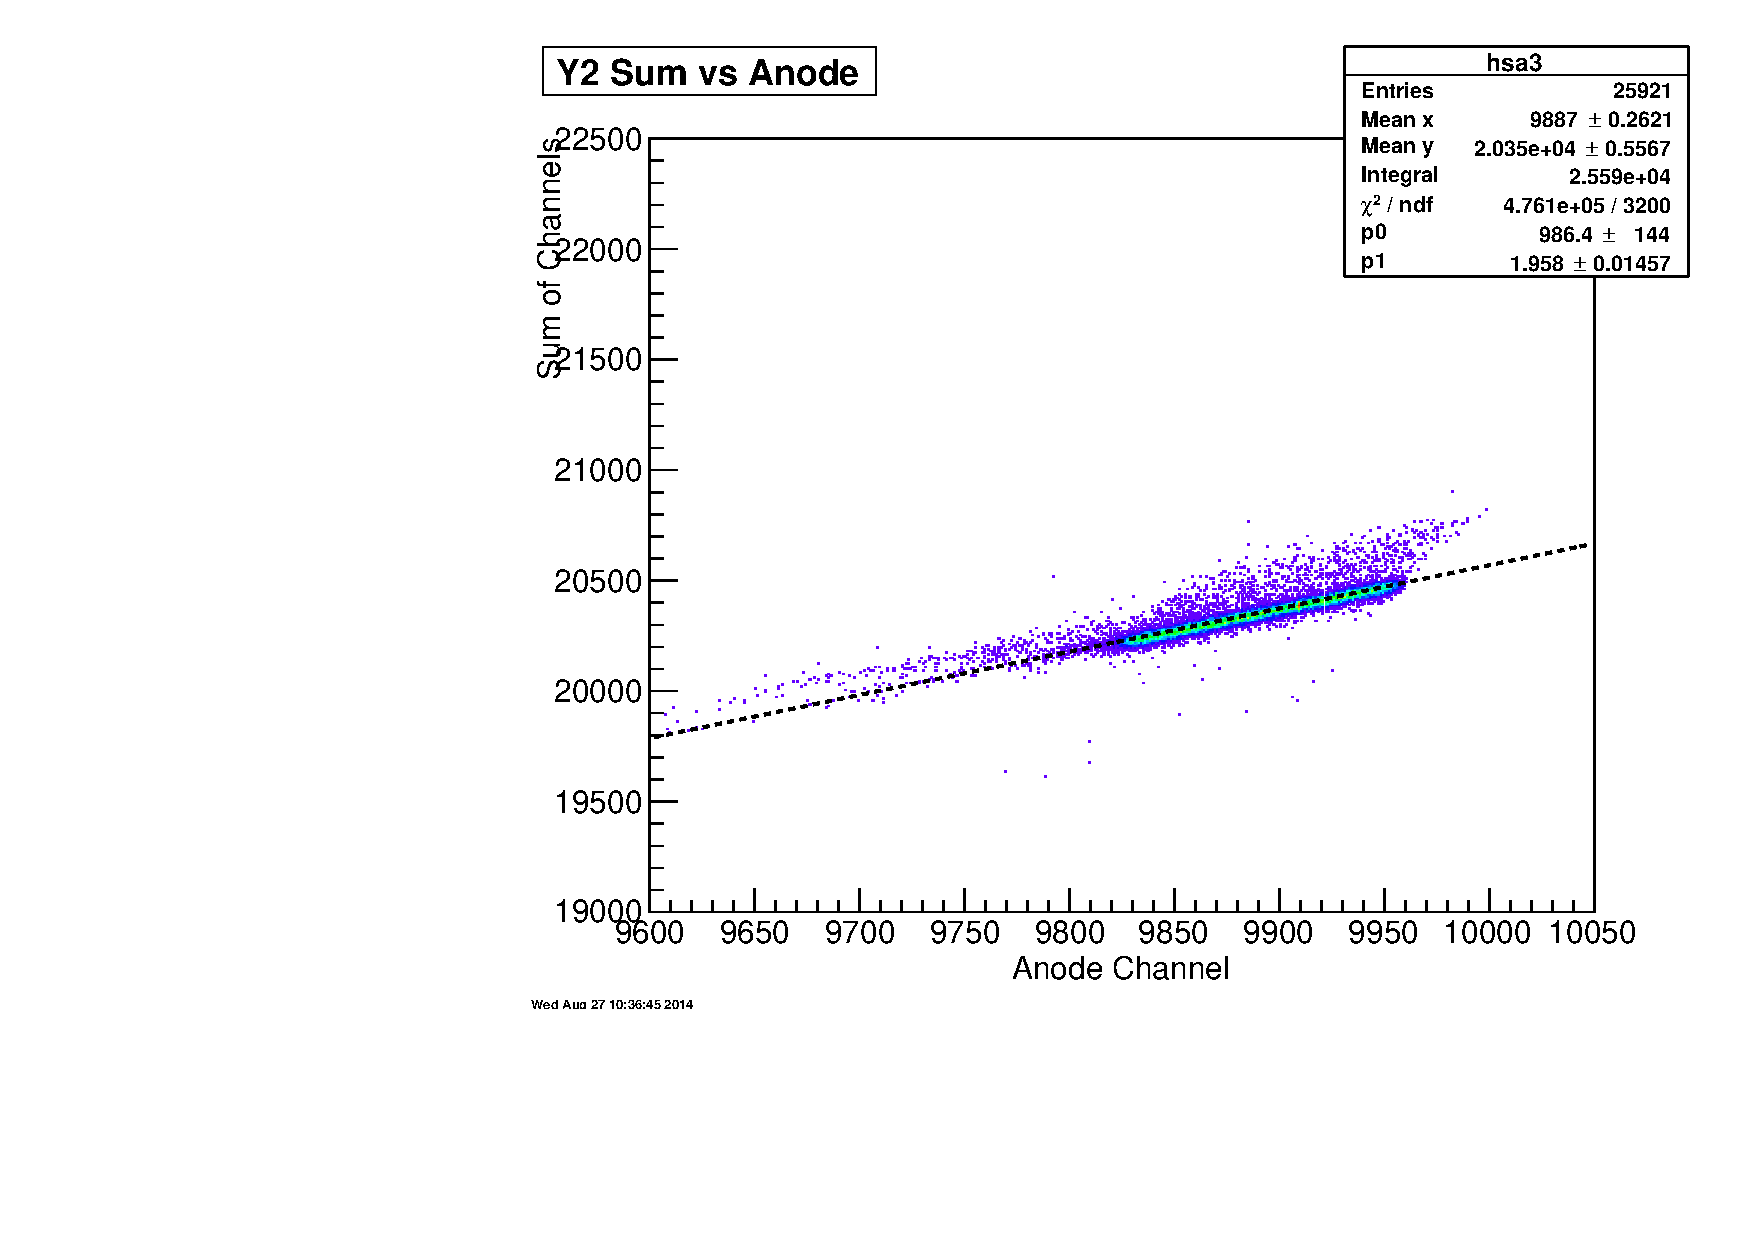
\includegraphics[width=0.48\textwidth, keepaspectratio]{run_480_hsa3_fit}\hspace{\fill}
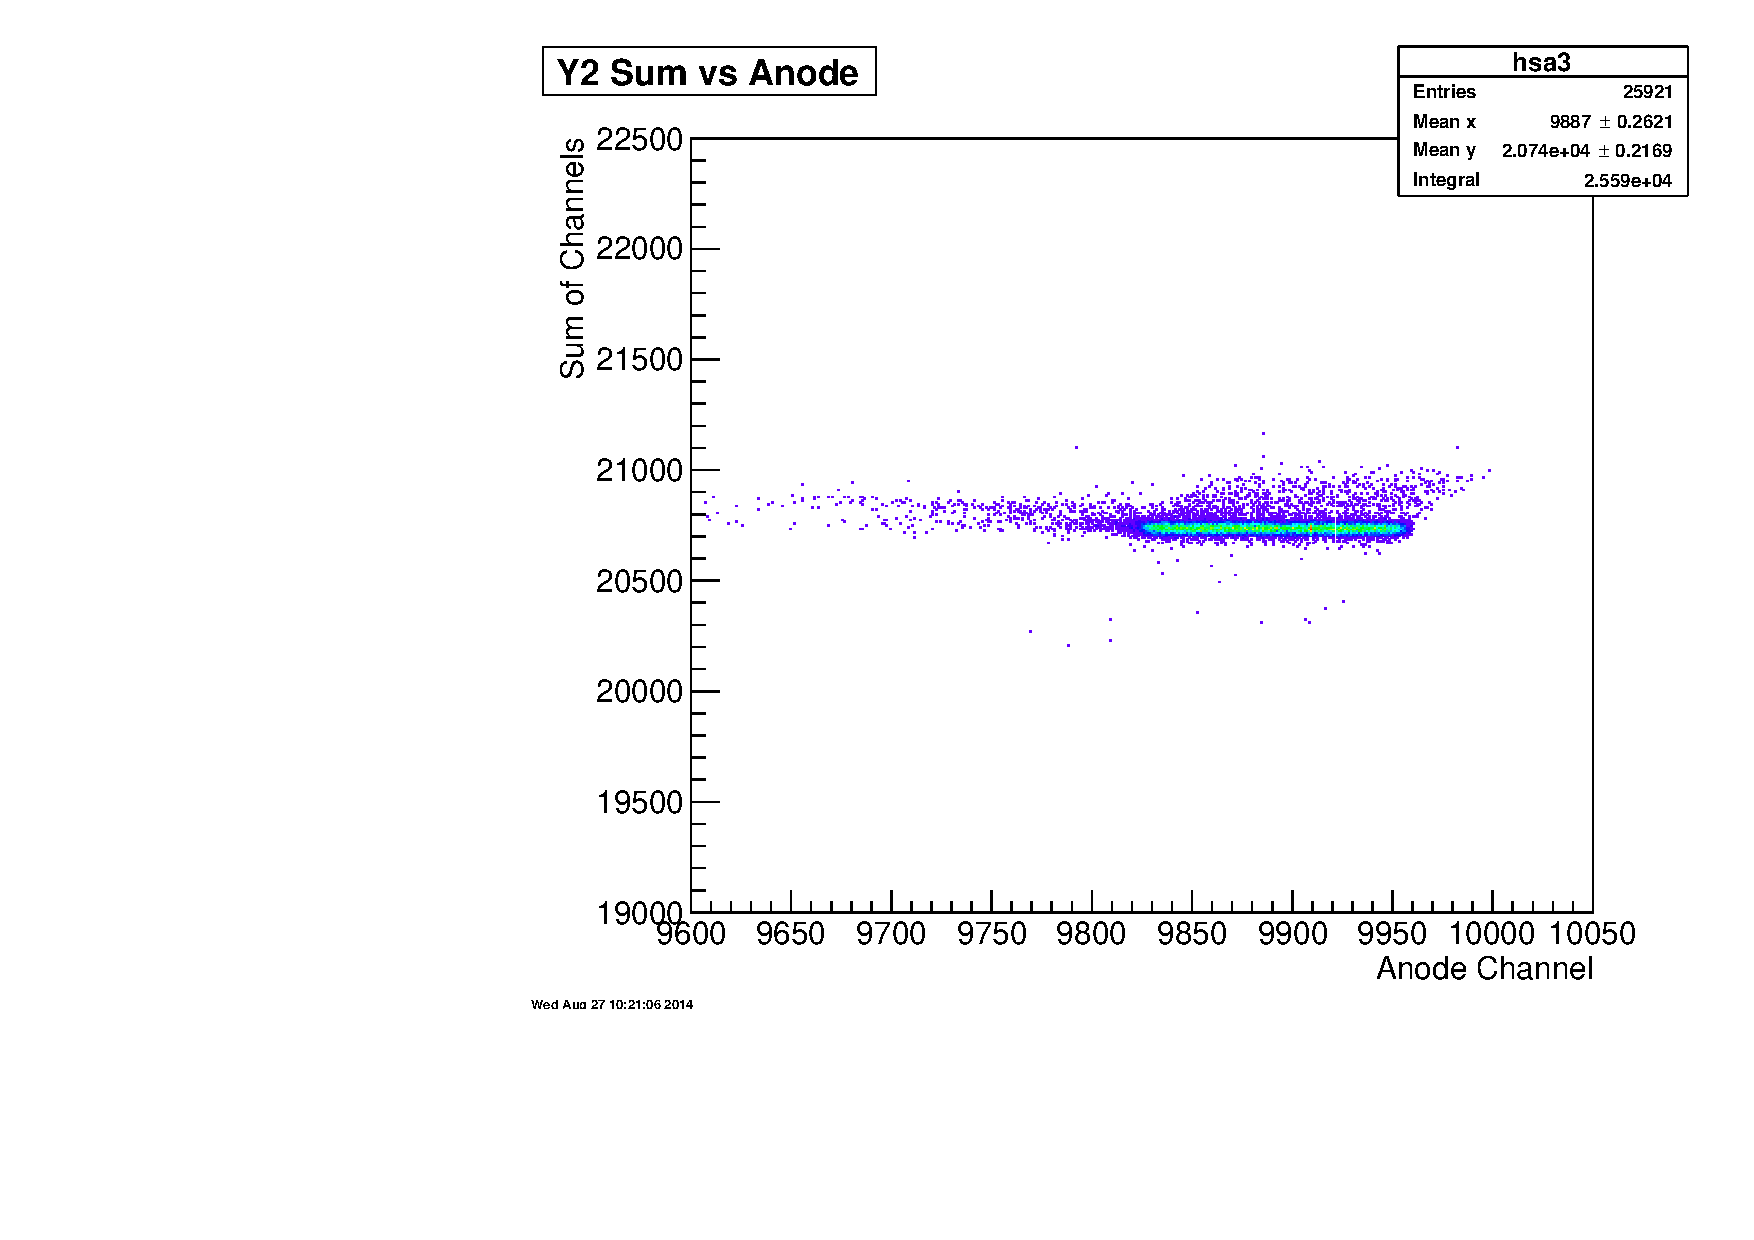
\includegraphics[width=0.48\textwidth, keepaspectratio]{run_480_hsa3_cor} \hspace{\fill}
\caption{The sum of the Y2 position signals are plotted against the sum of the anode signals.
(Left) The uncorrected correlation is plotted with a linear fit overlaid on the data.
(Right) The correlation is plotted after correcting for the slope.  The sum of the cathode signals is now constant.}
\label{hsa}
\end{figure}

\paragraph{Method}
The linear variation of the sum of the cathode signals as a function of the anode signal can be corrected with the following block of code.
\vspace{0.5\baselineskip}
\par\noindent
\begin{minipage}{\linewidth}
  \singlespace
\begin{lstlisting}[caption={Here the index \texttt{i} runs over 3--6, corresponding to the cathode signal pairs and \texttt{k} runs over 0--2, corresponding to the anode signal; as defined in Tables~\ref{TDC_signals} and \ref{position-andode}. The expression \texttt{(int)((i-3)/2)} has a value of 0 or 1 and selects the detector number. The expression \texttt{k+3*(int)((i-3)/2)} has a value of 0--5 
%1 or 4 
and selects the anode signal. See the text for further details.
},label=anode-cathode-eq]
if(a[k+3*(int)((i-3)/2)][1]>0) {
  xn[i-3][2]=xn[i-3][1]-(a[k+3*(int)((i-3)/2)][1]
                         *hasumcal[((i-3)*3)+k][1])/2;
  xn[i-3][2]+=hasumcal[((i-3)*3)+k][2]/2;
  xf[i-3][2]=xf[i-3][1]-(a[k+3*(int)((i-3)/2)][1]
                         *hasumcal[((i-3)*3)+k][1])/2;
  xf[i-3][2]+=hasumcal[((i-3)*3)+k][2]/2;
}
\end{lstlisting}
%xn-=(A[1+3*(int)((i-3)/2)]*hasumcal[i-3][1])/2-hasumcal[i-3][2]/2;
%xf-=(A[1+3*(int)((i-3)/2)]*hasumcal[i-3][1])/2-hasumcal[i-3][2]/2;
%\vspace{-1.3\baselineskip}
\end{minipage}
%\sloppy
\begin{sloppypar}

%If all three anode segments were connected independently, the ``1'' in the previous expression would be replaced with \texttt{k} and would run over 0--2.
The parameter array \texttt{hasumcal[((i-3)*3)+k][j]} holds three parameters for each possible combination of position and anode: the offset [0] and slope [1] of the linear fit, such as that  shown in Fig.~\ref{hsa}; and a second offset parameter [2].  The first two parameters are used to adjust the slope of the correlation to zero.  The second offset parameter is used to set the overall offset of the new, flattened distribution.  The sum of the position signals is arbitrarily shifted to 20,750, roughly corresponding to the average value of the uncalibrated sums of the cathode signals.  

\end{sloppypar}
\begin{table}
\centering  
\begin{tabular}{c...}
\hline
\multicolumn{1}{c}{Pair}& \multicolumn{1}{c}{Offset}& \multicolumn{1}{c}{Slope} & \multicolumn{1}{c}{Re-center} \\
\multicolumn{1}{c}{\texttt{i}}&\multicolumn{1}{c}{\texttt{hasumcal[i][0]}}&\multicolumn{1}{c}{\texttt{hasumcal[i][1]}}  &\multicolumn{1}{c}{\texttt{hasumcal[i][2]}}\\ \hline \hline
 0 & 1821.13 & 1.99218 & 18925.0 \\
 1 & 1824.38 & 1.99607 & 18925.8 \\
 2 & 1794.25 & 1.99819 & 18954.6 \\
 3 & 773.202 & 1.99094 & 19976.1 \\
 4 & 713.333 & 1.99371 & 20119.4 \\
 5 & 680.299 & 1.99967 & 20071.1 \\
 6 & 1539.11 & 2.01388 & 19171.5 \\
 7 & 1610.62 & 2.01017 & 19137.6 \\
 8 & 1474.61 & 2.01852 & 19202.7 \\
 9 & 660.381 & 2.00130 & 20095.6 \\
10 & 366.884 & 2.00641 & 20136.4 \\
11 & 1806.45 & 1.99139 & 20039.9 \\
 \hline 
\end{tabular}
\caption{Typical calibration constants for each of the twelve possible anode-cathode pairs (\texttt{i}).
The indices are the same as those shown in Table~\ref{position-andode}.
 Parameters are given for run 606. The slope parameter \texttt{hasumcal[i][1]} corrects the slope of the given cathode sum as a function of the given anode signal. 
%can be correlated with each of the three anode segment pairs (\texttt{k}); twelve combinations in total. The index runs from 0--11 and is defined by $(\texttt{i}-3)\times 3 + \texttt{k}$.
}
\label{anode-cathode-calib}
\end{table}


The results of this procedure are shown in Fig.~\ref{pos_cor}. This figure is generated with a command similar to the following (updated to reflect development of the analysis code).
\vsetroot
\begin{quote}
\begin{Verbatim}[firstnumber=0]
getressum("hsumz3","hxfxnznn3")
\end{Verbatim}
\end{quote}
\vsetnone
 By adding the same adjustment to each of the position signals, the difference of the position signals is unaffected.  The equations given in the next section show that by changing the value of the sum of the position signals, the calculated position will be altered.  However, using this method the sum of the position signals is made constant (as it should be). Furthermore, a linear position calibration will correct (undo) any change in the position caused by this refinement. The calibration constants obtained by the methods described in this section are stable and constant (on the order of 0.1\%) across all runs; this includes all detector settings and beam currents. The default calibration constants for the 2014 test are derived from run ; and the default for the 2015 tests are from run 606.

Inspection of Code Block~\ref{anode-cathode-eq} reveals that iterative application of this technique is additive. That is, if after applying the calibration constants, a test-fit reveals that the anode-dependence of the cathode sum is not completely removed, the new calibration constants are the sum of the old calibration constants. For example, if the initial fit has a slope of 2.0, and the subsequent test-fit has a slope of 0.01, the new calibration constant should be the sum of the two: 2.01. In all cases, the test fit should have a slope $\leq0.004$. Correspondingly, the sensitivity of the slope correction is about %$\frac{1}{500}$ 
1/500.
\begin{figure}
\centering
%\hspace{\fill}
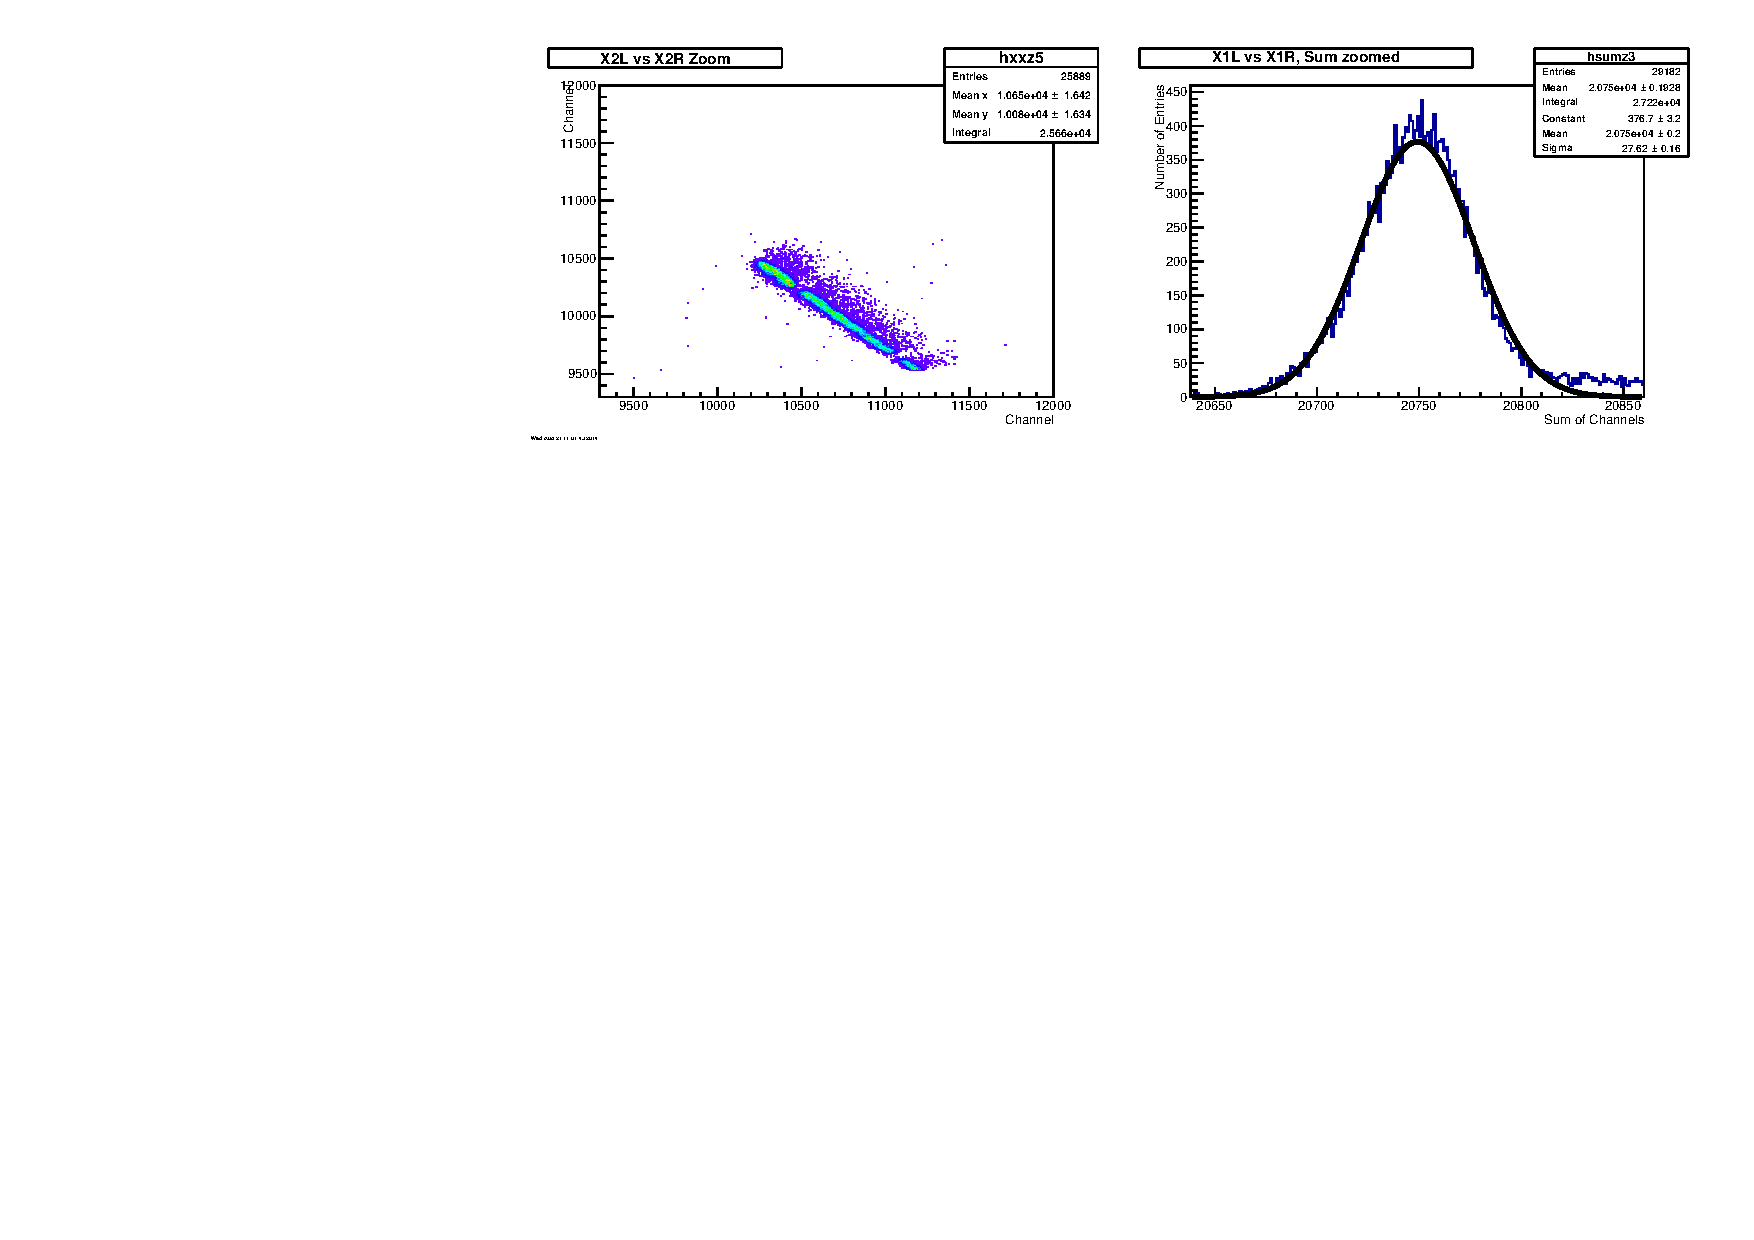
\includegraphics[width=\textwidth, keepaspectratio]{run_480_hxxz3}\hspace{\fill}
%\includegraphics[width=0.48\textwidth, keepaspectratio]{run_480_hsumz3_cor} \hspace{\fill}
\caption{(Left) Correlation plot the X2L and X2R position signals after correcting for the variations of the sum of the position signals as a function of the anode signal (cf. Fig.~\ref{reflect}). %\,(Left)).
  (Right) The sum of X2L and X2R (cf. Fig.~\ref{sum_fit}). %\,(Left)).
  Correcting for the anode variations reduces the width of the sum of the cathode signals by an average factor of $4.7\times$.}
\label{pos_cor}
\end{figure}

\subsection{Position}
\subsubsection{Definition}
The position signals may be  identified as $X_\mathrm{far}$ and $X_\mathrm{near}$, with ``far'' and ``near'' relative to one end of the detector.  To be consistent with Fig.~\ref{mask}, let us define ``near'' as the left-hand side of the detector in the $x$-direction and the bottom of the detector in the $y$-direction; both as viewed by the beam.  Recall, that the left side of the detector as viewed by the beam corresponds to the signals labeled X$n$R.
With the position derived from a delay line, the value of the delay is directly-proportional to the distance at which the ionization is detected.  As previously discussed, the sum of the position signals is effectively a measurement of the length of the delay line and is therefore constant.  %As a result, 
Combining these ideas, the position on the detector is proportional to $X_\mathrm{near}$.\footnote{Note that this is the opposite of the situation with a position-sensitive detector based on resistive division; i.e., with a position derived from resistive division, the position is proportional to the ``far'' signal divided by the sum.}
\begin{equation}
X\propto\left[\frac{X_\mathrm{near}}{(X_\mathrm{far}+X_\mathrm{near})}\right]
\label{detector_prop}
\end{equation}
The position on the detector may also be expressed in terms of the difference between he paired position signals.  When this difference is divided by the sum of the paired position signals, the result will vary over the interval $[-1,1]$.  The fractional position---that is, the position  over the interval $[0,1]$---can then be expressed as
%Express as a difference, the position on the detector may be rewritten as
\begin{equation}
\begin{split}
%X=&\frac{L}{2}\left[1+\frac{(X_\mathrm{far}-X_\mathrm{near})}{E}\right]
X=&\frac{L}{2}\left[1+\frac{(X_\mathrm{near}-X_\mathrm{far})}{(X_\mathrm{far}+X_\mathrm{near})}\right]
\label{detector_X}
\end{split}
\end{equation}
with $X=0$ corresponding to an event at the $X_\mathrm{near}$ end of the detector and $X=L$ corresponding to an event at the $X_\mathrm{far}$ end, where L is the length of the detector.  This is implemented in the code as follows.
%\pangram{10}
\vspace{0.5\baselineskip}
\par\noindent
\begin{minipage}{\linewidth}
\singlespace
\begin{lstlisting}[caption={Position definition with simple variables. The variable \texttt{xn} refers to the near side of the detector and \texttt{xf} refers to the far side of the detector.}]
x=(1/2.)*(1+((xn-xf)/(xf+xn)));//Position w/ xn@x=0 and xf@x=1 (delay).
\end{lstlisting}
\end{minipage}
%\pangram{10}
\vspace{0.5\baselineskip}
\par\noindent
\begin{minipage}{\linewidth}
\singlespace
\begin{lstlisting}[caption={Position definition with arrayed variables. Here the index \texttt{i} runs from 3--6 to cover the four pairs of positions. Each variable is a $4\times3$ array. The first index \texttt{i-3} corresponds to each position. The second index \texttt{k} corresponds to the calibration level: 0 for uncalibrated, 1 for partially calibrated, and 2 for fully calibrated.}]
for(Int_t k=0;k<3;k++) {
  x_sum [i-3][k]=xf[i-3][k]+xn[i-3][k];
  x_diff[i-3][k]=xn[i-3][k]-xf[i-3][k];
}
x[i-3][0]=(1/2.)*(1+((x_diff[i-3][2])/(x_sum[i-3][2])));
\end{lstlisting}
\end{minipage}

Again recalling that the sum of the positions signals is constant, we see from Eq.~\ref{detector_X} that the position 
%is also proportional 
has a linear relationship to the difference in the position signals.  This can be seen in Fig.~\ref{hdiffz} which plots the quantity $\textrm{X2R}-\textrm{X2L}$.  Referring to Table~\ref{TDC_signals}, we see that this difference corresponds to $(X_\mathrm{near}-X_\mathrm{far})$.  Also, when $X_\mathrm{far}$ is plotted against $X_\mathrm{near}$---as it is in Fig.~\ref{reflect}---we see that the position can also be obtained by projecting the distribution onto the line $y=-x$.
\begin{figure}
\centering
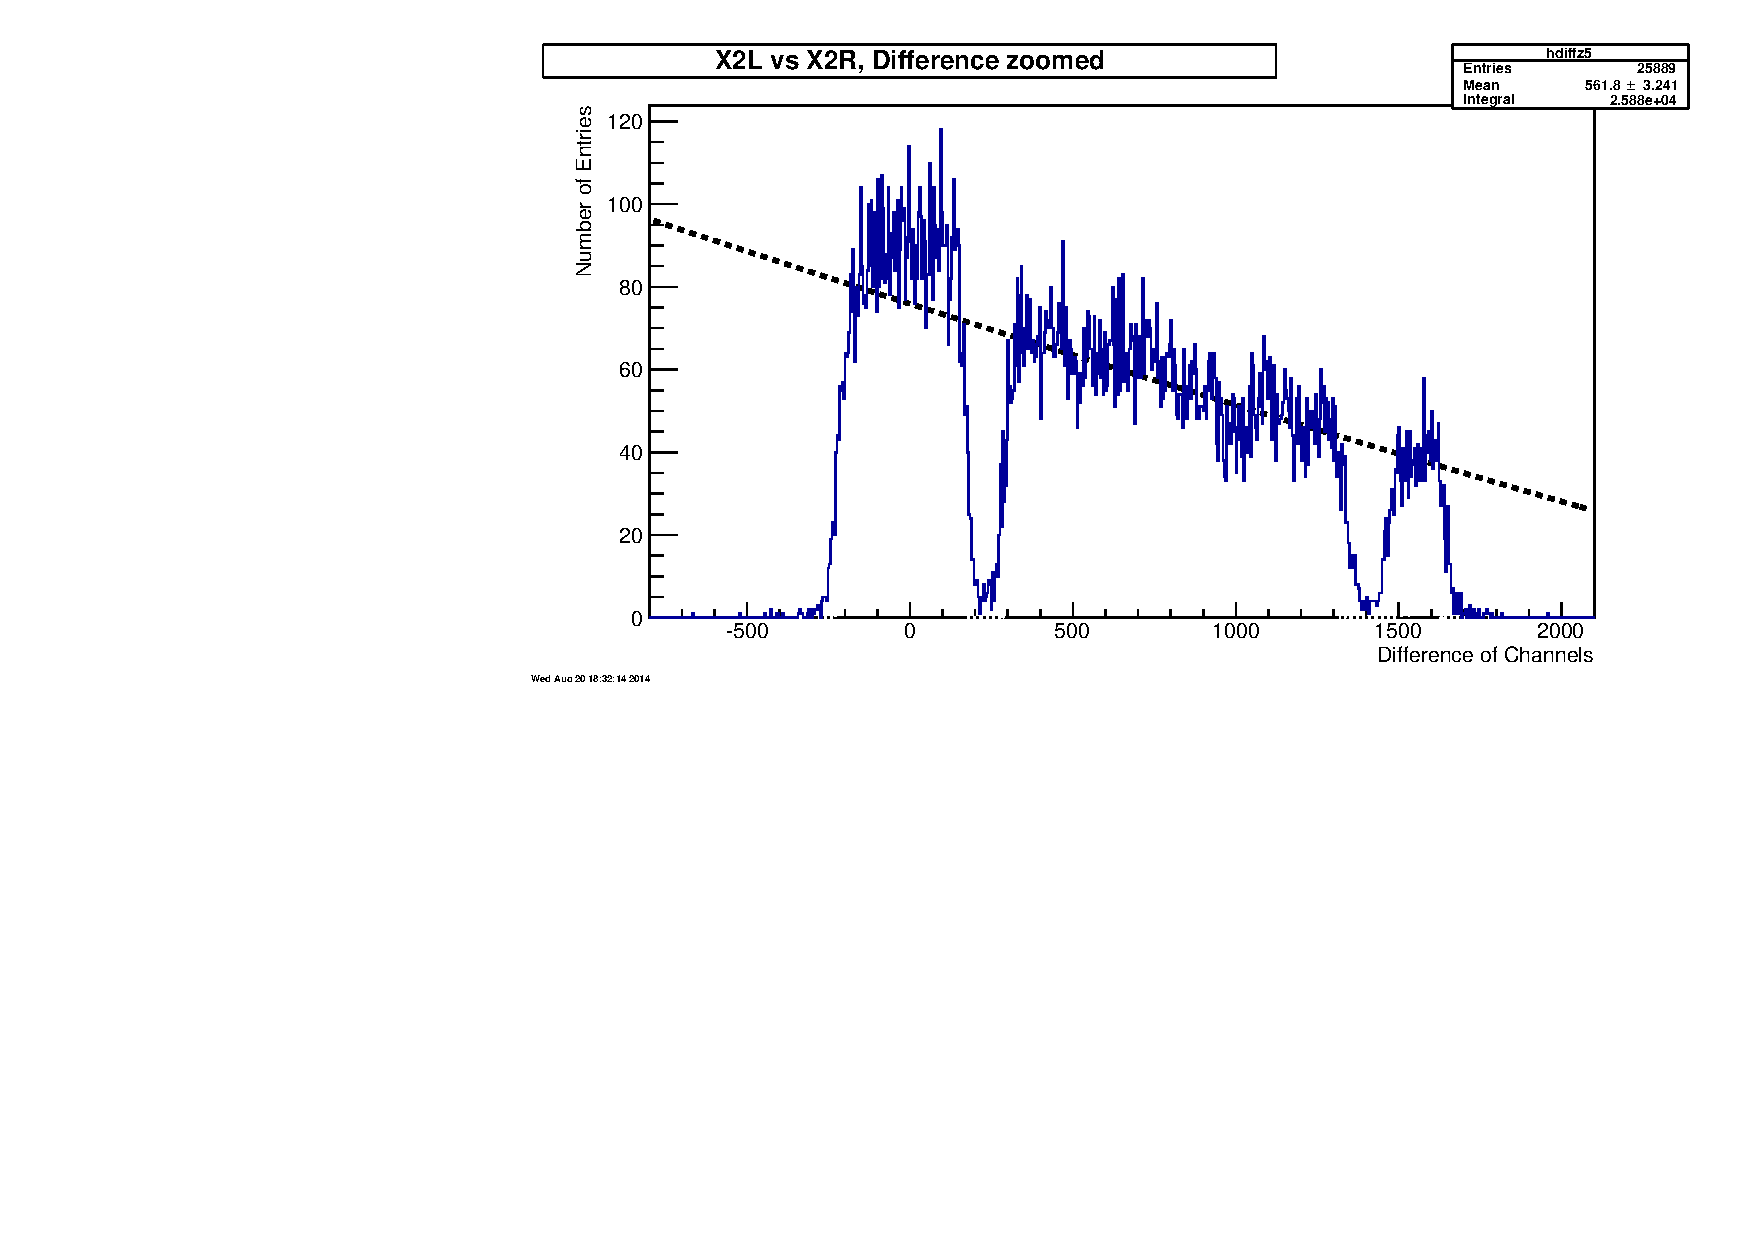
\includegraphics[width=\textwidth, keepaspectratio]{run_480_X2L_vs_X2Rg}
\caption{Example plot of the difference of paired position signals.  The gaps in the spectrum correspond to the mask shown in Fig.~\ref{mask}.  The overall distribution has been fit with a
 %$1/
$\csc^4 (\theta/2)$ function, characteristic of the Rutherford scattering cross section.
% (albeit flipped over the $y$-axix).
 The difference in channels has a linear relationship with the position.}%
\label{hdiffz}%
\end{figure}

\subsubsection{Reference Positions}
\label{cal_def}
The position calibration is based on the shadow cast by the masks shown in Figs.~\ref{mask} and \ref{mask2} onto the detector planes.  The $z$-positions of the detector planes is given in Table~\ref{zpos}.  The $z$-axis is defined by the central central beam trajectory, in this case corresponding to a polar angle of $\theta=30^\circ$ relative to the incident beam direction.
%This information is 
The $z$-positions given in Table~\ref{zpos} are based on the dimensions given in Fig.~\ref{rays} and the geometry of the detectors.  Knowing the dimensions of the mask and the separation of the detector planes allows the angle obscured by the features of the mask to be determined using the following equation
\begin{equation}
\theta=\arctan(x_m/z)
\label{eq:ang_in}
\end{equation}
where $x_m$ is the position of a specific feature of the mask relative to the central beam position.  Here $\theta$ is the scattering angle relative to the central beam trajectory.  Thus, the dimensions of the ``shadow'' on each of the detector planes can be calculated.    The results of these calculations are shown in Tables~\ref{xpos} and \ref{ypos} for the original mask; and Table~\ref{xpos2}  for the revised mask.  With the angle of the features determined and the $z$-position of the planes known, the calibration parameters can be calculated with the equation
\begin{equation}
x_p=z\tan(\theta)
\label{eq:ang_out}
\end{equation}
where $x_p$ is the position of a specific feature of the shadow cast by the mask on the detector plane.  The results of these calculations are shown in Tables~\ref{cal} and \ref{cal2}.  Both Eqs.~\ref{eq:ang_in} and \ref{eq:ang_out} assume that the mask is being illuminated by a point-source at the origin.
\begin{table}%
  \centering  
\begin{tabular}{r.}
\hline
\multicolumn{1}{c}{Plane} & \multicolumn{1}{c}{$z$-position} \\ \hline \hline
Target & 0.0 \\
Mask & 637.0 \\
Window (us)& 640.3\\
Window (ds)& 646.6\\
Y2 & 679.7 \\
Shield Y2 & 681.3 \\
A2 & 682.9 \\
Shield X2 & 684.5 \\
X2 & 686.1 \\
Y1 & 716.5 \\
Shield Y1 & 718.1 \\
A1 & 719.7 \\
Shield X1 & 721.3 \\
X1 & 722.9 \\ \hline 
\end{tabular}
\caption{Calculated $z$-positions of detector planes, including Kapton shields.  These positions are based on the measurements given in Fig.~\ref{rays} and the known spacing of the detector planes.  The three wire planes of each detector are separated by 3.18\,mm and the Kapton shields are centered between the wire planes.  The upstream (us) and downstream (ds) side of the frame for the Mylar window are also given.}
\label{zpos}
\end{table}

The Kapton shields are situated between the anode and the cathodes of each detector.  As such, the Kapton shields are perpendicular to the electric field lines between the electrode planes.  Thus, the Kapton shields do not block out the same angle on each detector, rather they put limits on the measured position.  The Kapton shields also produce partial charge collection for particle trajectories at the edges of the detector with scattering angles $\theta \neq 0$.  The particle trajectories (and therefore the ionization paths) cover transverse extents $\delta x$, $\delta y$, and $\delta \rho$ given by %\textit{<this does not include the azimuthal angle and needs to be updated>}
\begin{equation}
  \begin{split}
\delta x=&\Delta z\tan(\theta)\cos(\varphi)\\
\delta y=&\Delta z\tan(\theta)\sin(\varphi)\\
\delta \rho=&\sqrt{\delta x^2 + \delta y^2}
=\Delta z\tan(\theta)
\label{eq:ang_error}
\end{split}
\end{equation}
where $\Delta z$ is the separation between the anode and cathode (3.18\,mm) and $\varphi$ is the azimuthal angle of the incident particle.  For example, a trajectory intercepting the right-hand edge of the Y2 shield has a polar angle of $\theta=3.03^\circ$.  At this angle, the trajectory has a transverse extent of $\delta \rho = 0.17$\,mm between the anode and cathode. %This smearing out of the
%For trajectories in the region of the Kapton shields, part of the transverse extent of the
In this example, only half of the ionization %path will not
will be collected by the cathode. %electrodes.
The transverse extent of particle trajectories could also contribute to %also leads to
 an angle-dependent degradation of the position resolution.  However, in the extreme case given in the previous example, the transverse extent of the trajectory is small compared to the position resolution of the detector.

The transverse extent of particle trajectories introduces a small ambiguity as to what is meant by the measured position.  The position of a particle trajectory at the cathode plane will differ from the position of the particle trajectory at the anode plane by $\delta \rho$ given in Eq.~\ref{eq:ang_error}.  For example, the relation between the $y$-position of a particle trajectory at the Y2 cathode plane and the A2 anode plane is given by 
$y|_{z=\textrm{A2}}=y|_{z=\textrm{Y2}}+\delta y=y|_{z=\textrm{Y2}+\Delta z}$. %\\ 
%$x|_{z=\textrm{Y2 Shield}}=x|_{z=\textrm{A2}}=-\delta x/2 =x|_{z=\textrm{Y2}}+\delta x/2$
The average position of the charge collected from particle trajectory (i.e., the measured position) will be equal to the position of the particle trajectory half-way between the detector planes.  This position in the $z$-direction corresponds to the position of the Kapton shield.  \textbf{Therefore, the $\boldsymbol{x}$- and $\boldsymbol{y}$-positions of the calibration features given Tables~\ref{cal} and \ref{cal2} are evaluated at the $z$-positions of the respective intra-electrode Kapton shields.}

\paragraph{Original Mask}
Tables~\ref{xpos} and \ref{ypos} give the $x$- and $y$-positions, respectively, of the calibration features of the original mask. Table~\ref{cal} gives the reference positions of the calibration features at each cathode plane.

\begin{table}%
\centering 
\begin{tabular}{ll....}
\hline
&\multicolumn{4}{c}{$x$-position}\\ \cline{3-4}
Feature & No. & \multicolumn{1}{c}{Rel. to shield} & \multicolumn{1}{c}{Rel. to beam} &  \multicolumn{1}{c}{Angle} &\multicolumn{1}{c}{$z$-position}\\ \hline \hline
Left edge of shield & 0 & 0.0 & -118.0 & \multicolumn{1}{c}{\textit{multiple}} &\multicolumn{1}{c}{\textit{multiple}} \\
Left edge of mask (curve) & 1 & 68.3 & -49.8 & -4.5 &637.0 \\
Left side of left mask & 2 & 87.0 & -31.0 & -2.8 &637.0 \\
Right side of left mask & 3 & 92.0 & -26.0 & -2.3 &637.0 \\
Left side of right mask & 4 & 137.0 & 19.0 & 1.7 &637.0 \\
Right side of right mask & 5 & 142.0 & 24.0 & 2.2 &637.0 \\
Right edge of shield & 6 & 154.0 & 36.0 & \multicolumn{1}{c}{\textit{multiple}} &\multicolumn{1}{c}{\textit{multiple}} \\
Right edge of window & 7 & 152.0 & 34.0 & 3.0 &646.6 \\
\hline
\end{tabular}
\caption{Calculated $x$-positions of calibration features; cf. Fig.~\ref{mask}.  Distances are given relative to the ``right'' of the detector (as seen by the beam). This position corresponds to the edge of the Kapton shield. Positions and angles  relative to the center of the circular aperture of the mask (i.e. the beam spot) are also given.}
\label{xpos}
\end{table}

\begin{table}%
\centering 
\begin{tabular}{ll....}
\hline
&\multicolumn{4}{c}{$y$-position}\\ \cline{3-4}
Feature & No. & \multicolumn{1}{c}{Rel. to shield} & \multicolumn{1}{c}{Rel. to beam} & \multicolumn{1}{c}{Angle} &\multicolumn{1}{c}{$z$-position}\\ \hline \hline
Bottom of shield & 1 & 0.0 & -27.0 & \multicolumn{1}{c}{\textit{multiple}} &\multicolumn{1}{c}{\textit{multiple}} \\
Bottom of lower mask & 2 & 12.0 & -15.0 & -1.3 &637.0 \\
Top of lower mask & 3 & 17.0 & -10.0 & -0.9 &637.0 \\
Bottom of upper mask & 4 & 37.0 & 10.0 & 0.9 &637.0 \\
Top of upper mask & 5 & 42.0 & 15.0 & 1.3 &637.0 \\
Top of shield & 6 & 54.0 & 27.0 & \multicolumn{1}{c}{\textit{multiple}} &\multicolumn{1}{c}{\textit{multiple}} \\
\hline
\end{tabular}
\caption{Calculated $y$-positions of calibration features; cf. Fig.~\ref{mask}. Distances are given relative to the ``bottom'' of the detector (as seen by the beam). This position corresponds to the edge of the Kapton shield.  Positions and angles  relative to the center of the circular aperture of the mask (i.e. the beam spot) are also given.}
\label{ypos}
\end{table}


\begin{table}%
\centering
\begin{tabular}{lc....}
\hline
Feature&No. & \multicolumn{1}{c}{Y2} & \multicolumn{1}{c}{X2} & \multicolumn{1}{c}{Y1} & \multicolumn{1}{c}{X1} \\ \hline \hline
\textit{leftmost}&1 & 0.0 & 64.5 & 0.0 & 61.7\\
Mask&2 & 11.0 & 84.7 & 10.1 & 82.9\\
Mask&3 & 16.3 & 90.1 & 15.7 & 88.6\\
Mask&4 & 37.7 & 138.4 & 38.3 & 139.5\\
Mask&5 & 43.0 & 143.8 & 43.9 & 145.2\\
Mask&6 & 54.0 & 154.0 & 54.0 & 154.0\\
\hline
\end{tabular}
\caption{Calculated calibration parameters for each cathode plane.}
\label{cal}
\end{table}

\paragraph{Revised Mask}
Tables~\ref{xpos2} and \ref{ypos} give the $x$- and $y$-positions of the calibration features of the revised mask. Table~\ref{cal2} gives the reference positions of the calibration features at each cathode plane.

\begin{table}[ht!]%
\centering 
\hspace{\fill}
\begin{tabular}{c...}
\hline
&\multicolumn{2}{c}{$x$-position}\\ \cline{2-3}
 Col. & \multicolumn{1}{c}{Rel. to shield} & \multicolumn{1}{c}{Rel. to beam} & \multicolumn{1}{c}{Angle} \\ \hline \hline
 1 & 71.0 & -47.0 & -4.2  \\
2 & 75.0 & -43.0 & -3.9  \\
3 & 79.0 & -39.0 & -3.5  \\
4 & 83.0 & -35.0 & -3.1  \\
5 & 87.0 & -31.0 & -2.8  \\
6 & 91.0 & -27.0 & -2.4  \\
7 & 95.0 & -23.0 & -2.1  \\
8 & 99.0 & -19.0 & -1.7 \\
9 & 103.0 & -15.0 & -1.3 \\
10 & 107.0 & -11.0 & -1.0  \\
11 & 111.0 & -7.0 & -0.6  \\
12 & 115.0 & -3.0 & -0.3 \\
13 & 119.0 & 1.0 & 0.1  \\
14 & 123.0 & 5.0 & 0.4  \\
15 & 127.0 & 9.0 & 0.8  \\
16 & 131.0 & 13.0 & 1.2  \\
17 & 135.0 & 17.0 & 1.5  \\
18 & 139.0 & 21.0 & 1.9 \\
19 & 143.0 & 25.0 & 2.2  \\
20 & 147.0 & 29.0 & 2.6  \\
21 & 151.0 & 33.0 & 3.0  \\
\hline
\end{tabular}
\hspace{\fill}
\begin{tabular}{c...}
\hline
&\multicolumn{2}{c}{$y$-position}\\ \cline{2-3}
 Row. & \multicolumn{1}{c}{Rel. to shield} & \multicolumn{1}{c}{Rel. to beam} & \multicolumn{1}{c}{Angle} \\ \hline \hline
 1   & 3.0 & -24.0 & -2.2  \\
 2   & 7.0 & -20.0 & -1.8  \\
\textit{skip}   & 11.0 & -16.0 & -1.4  \\
 3 &   15.0 & -12.0 & -1.1 \\
 4 &   19.0 & -8.0 & -0.7  \\
 5 &   23.0 & -4.0 & -0.4  \\
 6 &   27.0 & 0.0 & 0.0  \\
 7 &   31.0 & 4.0 & 0.4  \\
 8 &   35.0 & 8.0 & 0.7  \\
 9 &   39.0 & 12.0 & 1.1  \\
 10 &   43.0 & 16.0 & 1.4  \\
 11 &   47.0 & 20.0 & 1.8  \\
 12 &   51.0 & 24.0 & 2.2  \\
\hline
\end{tabular}
\hspace{\fill}
\caption{Calculated $x$-positions of calibration features; cf. Fig.~\ref{mask2}.  Distances are given relative to the ``right'' of the detector (as seen by the beam). This position corresponds to the edge of the Kapton shield. Positions and angles  relative to the center of the circular aperture of the mask (i.e. the beam spot) are also given. Calculated $y$-positions of calibration features; cf. Fig.~\ref{mask2}. Distances are given relative to the ``bottom'' of the detector (as seen by the beam). This position corresponds to the edge of the Kapton shield.  Positions and angles  relative to the center of the circular aperture of the mask (i.e. the beam spot) are also given.}
\label{xpos2}
\end{table}

\begin{table}[ht]%
\centering
\hspace{\fill}
\begin{tabular}{c..}
\hline
Col. & \multicolumn{1}{c}{X1} & \multicolumn{1}{c}{X2} \\ \hline \hline
1 & 67.5 & 64.8\\
2 & 71.8 & 69.3\\
3 & 76.1 & 73.8\\
4 & 80.4 & 78.4\\
5 & 84.7 & 82.9\\
6 & 89.0 & 87.4\\
7 & 93.3 & 92.0\\
8 & 97.6 & 96.5\\
9 & 101.9 & 101.0\\
10 & 106.2 & 105.5\\
11 & 110.5 & 110.1\\
12 & 114.8 & 114.6\\
13 & 119.1 & 119.1\\
14 & 123.4 & 123.7\\
15 & 127.7 & 128.2\\
16 & 132.0 & 132.7\\
17 & 136.3 & 137.2\\
18 & 140.6 & 141.8\\
19 & 144.9 & 146.3\\
20 & 149.2 & 150.8\\
21 & 153.5 & 155.4\\
\hline
\end{tabular}
\hspace{\fill}
\begin{tabular}{c..}
\hline
Row. & \multicolumn{1}{c}{Y1} & \multicolumn{1}{c}{Y2} \\ \hline \hline
1 & 1.3 & -0.1\\
2 & 5.6 & 4.5\\
\textit{skip} & 9.9 & 9.0\\
3 & 14.2 & 13.5\\ \hline
4 & 18.4 & 18.0\\
5 & 22.7 & 22.5\\
6 & 27.0 & 27.0\\
7 & 31.3 & 31.5\\
8 & 35.6 & 36.0\\ \hline
9 & 39.8 & 40.5\\
10 & 44.1 & 45.0\\
11 & 48.4 & 49.5\\
12 & 52.7 & 54.1\\
\hline
\end{tabular}
\hspace{\fill}
\caption{Calculated calibration parameters for each cathode plane. Note that rows 1 and 12 are outside the acceptance of detector 2.}
\label{cal2}
\end{table}

\subsubsection{Method}
The most important part of the preceding gain-matching procedures of the calibration process is removal of the anode dependance from cathode sums. In that procedure, the dependence had to be removed for each anode individually. In a similar manner, the position calibrations must be applied to each position based on the corresponding anode segment. Therefore, each data set will have twelve sets of position calibration constants. The procedure for determining the calibration constants is illustrated in Fig.~\ref{peakfit}.

\begin{figure}[ht!]%
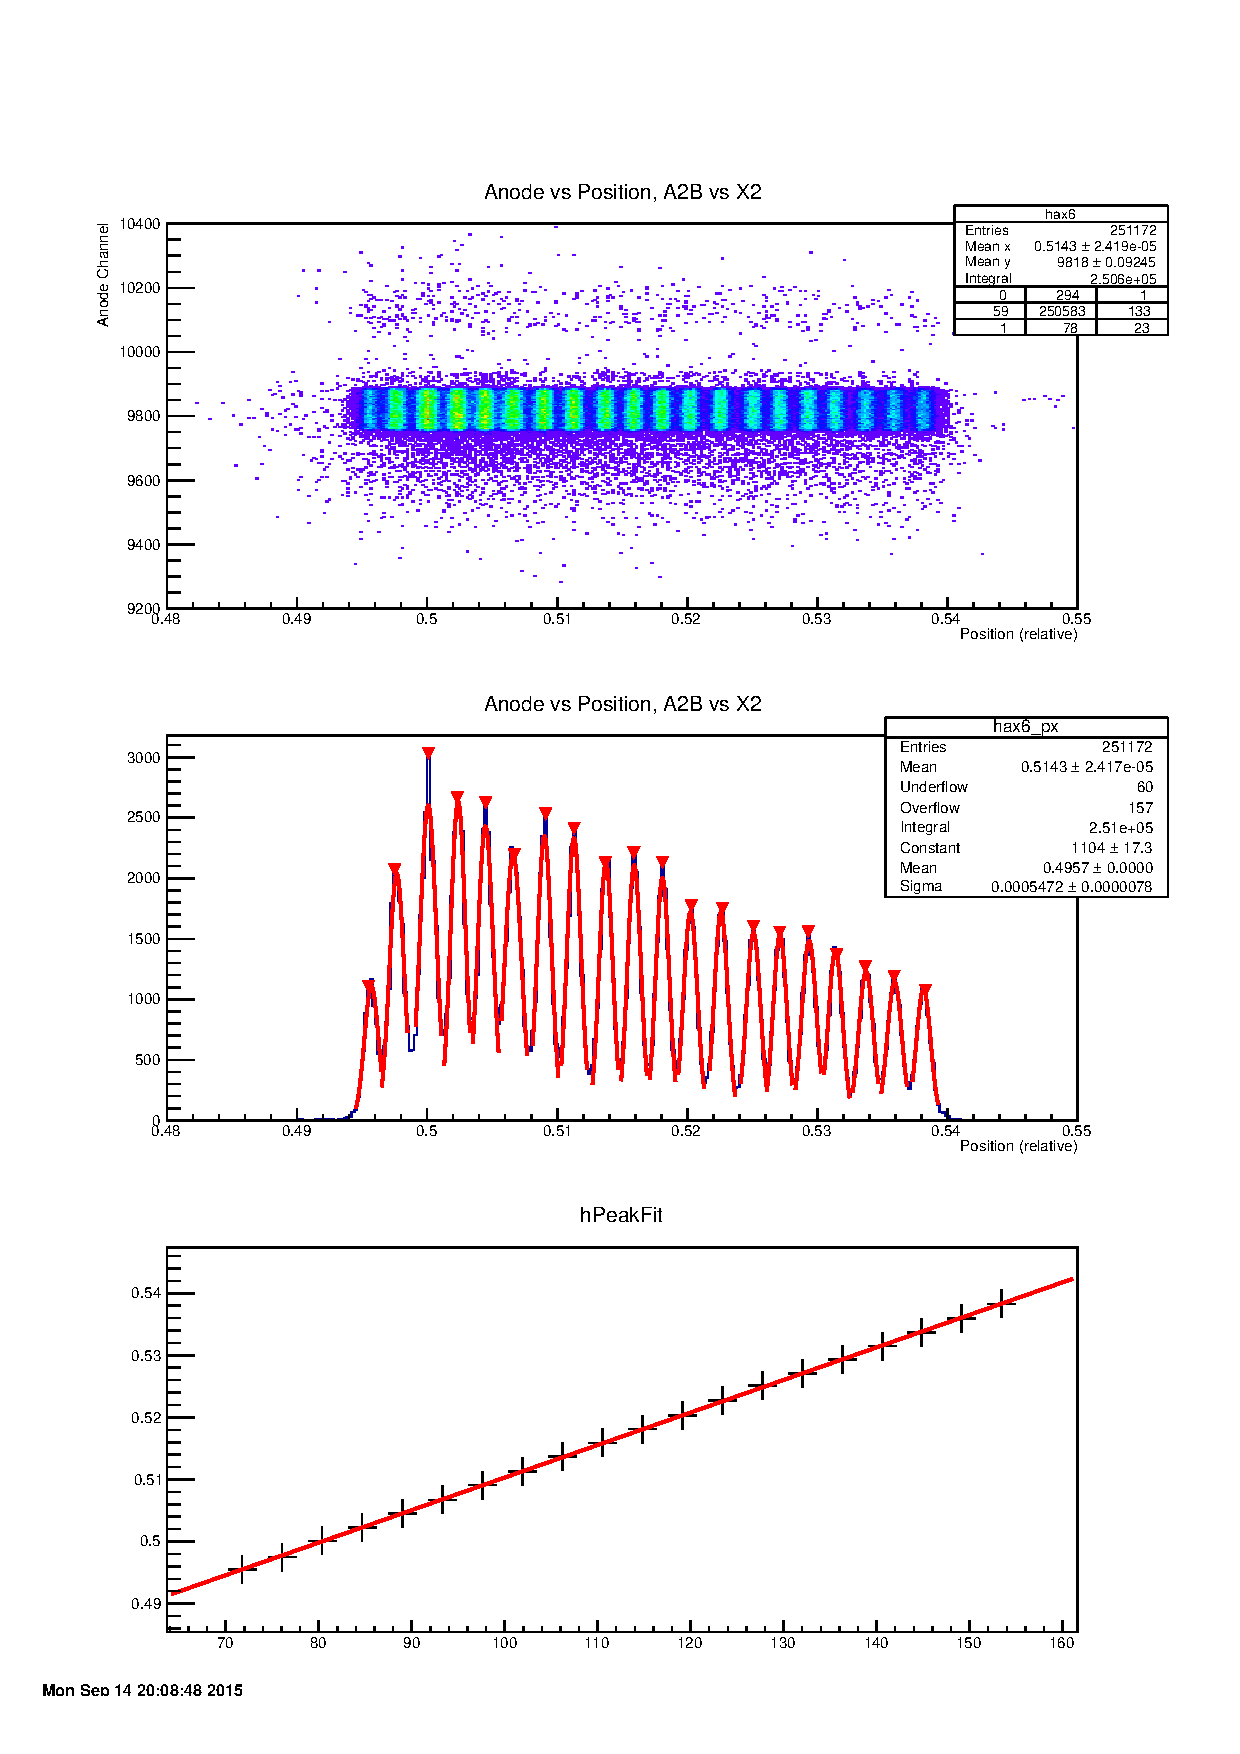
\includegraphics[width=\textwidth,height=0.8\textheight,keepaspectratio]{run_606_peakfit}%
\caption{Illustration of the position calibration technique. The 2D histogram is show in the top panel, in this case it is the $x$-position of detector 2 plotted against the bottom anode signal (also of detector 2). The middle panel shows the $x$-projection of the 2D histogram, that is the $x$-position spectrum gated on anode A2B. The location of the peaks have been identified (the width of the peaks has also been measured). The bottom panel shows how the calibration parameters are generated. The measured positions of the peaks (from the middle panel) are plotted as a function of the known peak positions from Table~\ref{cal2}. A linear fit is applied to the relationship, thus yielding the calibration constants show in Table~\ref{position-calib} for this position-anode combination.
%\enlargethispage{1in}
}%
\label{peakfit}%
\end{figure}

The calibration parameters are determined by comparing the location of the peaks in the spectrum with the known location of the projected features of the mask, which are given in Tables \ref{xpos} and \ref{ypos} (for the April 2014 runs) and in Table~\ref{xpos2} (for the April 2015 runs). As discussed in section \ref{fit}, the position of the peaks in the spectra can be determined using the following routine.
\vsetroot
\begin{quote}
\begin{Verbatim}[firstnumber=0]
peakfitx("hax6","cal/X2_grid.lst")
\end{Verbatim}
\end{quote}
Fig.~\ref{peakfit} shows part of the output of this routine. In the top panel, the 2D histogram \texttt{hax6} is given. 
This is a plot of the anode AB2 signal as a function of the uncalibrated $x$-position. 
The middle panel shows the 1D $x$-projection of the 2D histogram in the top panel. This spectrum, \texttt{hax6\_px}, corresponds to the $x$-position in coincidence with anode AB2. The peaks which have been identified using the subroutine  \texttt{findpeaks()} are indicated by the red triangles and the non-overlapping Gaussian fits determined by the subroutine \texttt{gfindpeaks()} are indicated by the solid red lines. Fig.~\ref{decon} shows a portion of the output from the third step of the peak-finding routine. The fitting range of the first three peaks are shown. As in the middle panel of Fig.~\ref{peakfit}, the peaks found by the subroutine  \texttt{findpeaks()} are indicated by red triangles and the non-overlapping Gaussian fits are indicated by the solid red lines. The global fit calculated by \texttt{decon()} is show by the solid green line. The individual Gaussian fits which make up the global fit are shown by the dashed black lines. By inspection the peak center revealed by the three different techniques is different---in particular for the first peak, located near $x=0.496$.

\begin{figure}
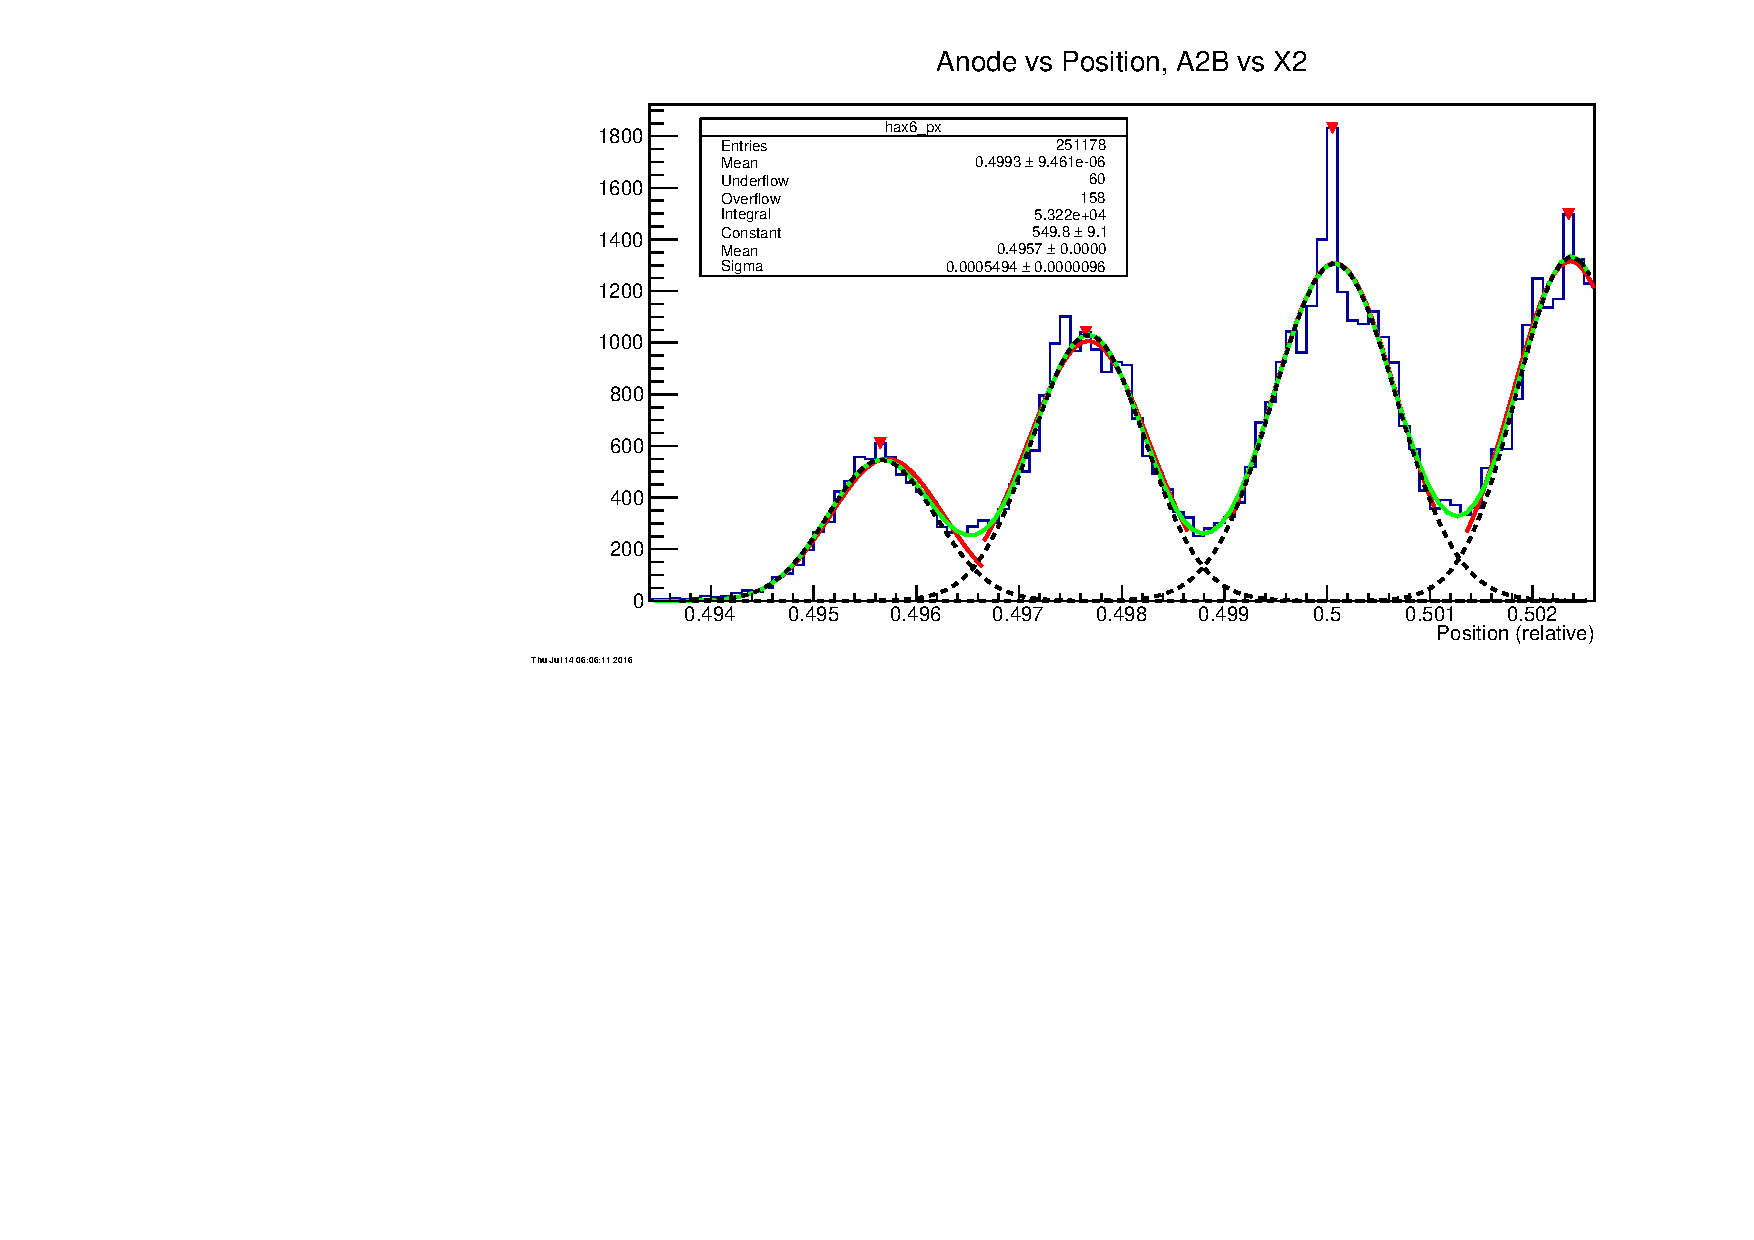
\includegraphics[width=\textwidth,keepaspectratio]{run_606_decon}%
\caption{Illustration of the peak-finding routine used in position calibration.}%
\label{decon}%
\end{figure}

It is the output of the \texttt{decon()} subroutine---that is, the center of the individual Gaussian fits---that are used as the peak positions that are to be calibrated. These positions are plotted on the $y$-axis of the bottom panel in Fig.~\ref{peakfit}. 
The known positions of the peaks are read in from a file, when specified as the second argument of the commands \texttt{peakfit()}, \texttt{peakfits()}, or \texttt{peakfity()}. 
The known positions are plotted on the $x$-axis of the bottom panel in Fig.~\ref{peakfit}. A linear fit is made between these two sets of points, which gives the calibration parameters for the particular andoe-position pair. For convenience, the following command can be used to save the calculated linear fit calibration parameters to file, to be read in during sorting.

\begin{quote}
\begin{Verbatim}[firstnumber=0]
writetemp("cal/run_606_XY.cal",-1,"temp_inv.lst",0,1,1,12,0)
\end{Verbatim}
\end{quote}


The calibration parameters are applied to the uncalibrated data using the code shown in Code Block~\ref{cal-code}. %with the following block of code.
The uncalibrated positions are given by Eq.~\ref{detector_X} with $L=1$ and are therefore unitless.  Naively, the uncalibrated positions should cover the range of 0--1, but inspection of the top  panel in Fig.~\ref{peakfit} shows the rage is closer to 0.49--0.54. In either case, 
the standard fit of the relationship shown in the bottom panel of Fig.~\ref{peakfit} will give calibration parameters  in terms of mm/unit~position.
In these terms, a typical calibration constant would be -0.00119\,mm/unit~position. % with an offset of 0.471\,mm.
 Instead of using calibration constants that are small compared to 1, the inverse of the usual calibration is used, as shown in Code Block~\ref{cal-code}. Typical values for the (inverted) calibration constants are given in Table~\ref{position-calib}.
\vspace{0.5\baselineskip}
\par\noindent
\begin{minipage}{\linewidth}
\singlespace
\begin{lstlisting}[caption={Position calibration procedure. The index \texttt{i} runs over 3--6, corresponding to each of the four positions. Each position has a separate set of calibration parameters for each anode segment. The calibration parameters are stored in the array $12\times2$ \texttt{hxcal[][]}. Typical calibration parameters are given in Table~\ref{position-calib}.},label={cal-code}]
for(int k=0;k<3;k++) {
  if(a[k+3*(int)((i-3)/2)][1]>0)
    x[i-3][1]=(x[i-3][0]*hxcal[((i-3)*3)+k][0])+hxcal[((i-3)*3)+k][1];
}
\end{lstlisting}
\end{minipage}

\begin{table}
\centering  
\begin{tabular}{c..}
\hline
\multicolumn{1}{c}{Pair}& \multicolumn{1}{c}{Slope}& \multicolumn{1}{c}{Offset} \\
\multicolumn{1}{c}{\texttt{i}}&\multicolumn{1}{c}{\texttt{hxcal[i][0]}}&\multicolumn{1}{c}{\texttt{hxcal[i][1]}}\\ \hline \hline
 0 & 1878.17 & -864.607 \\
 1 & 1851.11 & -851.023 \\
 2 & 1875.96 & -863.33 \\
 3 & 1734.11 & -843.706 \\
 4 & 1633.01 & -790.65 \\
 5 & 1645.94 & -794.028 \\
 6 & 1919.17 & -879.249 \\
 7 & 1905.22 & -872.308 \\
 8 & 1909.97 & -874.645 \\
 9 & 1783.57 & -867.804 \\
10 & 1620.39 & -784.588 \\
11 & 1586.56 & -764.344 \\
 \hline 
\end{tabular}
\caption{Typical calibration constants for each of the twelve possible anode-cathode pairs (\texttt{i}). Parameters are given for run 606. 
%can be correlated with each of the three anode segment pairs (\texttt{k}); twelve combinations in total. The index runs from 0--11 and is defined by $(\texttt{i}-3)\times 3 + \texttt{k}$.
}
\label{position-calib}
\end{table}




